\documentclass[pdflatex,sn-basic]{sn-jnl}
% Official Springer Nature author template v3.1 (December 2024).
% Single-column submission layout; production determines the published layout.
\usepackage{amsmath,amssymb,booktabs,graphicx,microtype,xcolor}
\usepackage{capt-of,enumitem,longtable,array,placeins}
\providecommand{\bibinfo}[2]{}
\renewcommand{\bibinfo}[2]{}
\hypersetup{hidelinks}
% Keep journal placement notes in the right margin on both odd and even pages.
% This changes note placement only; the publisher's page geometry is retained.
\makeatletter
\@mparswitchfalse
\makeatother
\normalmarginpar
\raggedbottom
\widowpenalty=10000
\clubpenalty=10000
\setlength{\emergencystretch}{2em}
\newcommand{\fedd}{f_{\mathrm{Edd}}}
\newcommand{\mbh}{M_{\mathrm{BH}}}
\newcommand{\mseed}{M_{\mathrm{seed}}}
% Local table fragments are expanded into the single uploaded manuscript.
\newcommand{\tableinput}[1]{\csname @@input\endcsname #1 }

\begin{document}
\articletype{Research article}
\title[High-redshift black-hole growth requirements]{Growth Requirements for High-Redshift Black Holes: A JWST-Era Catalogue}
\author*{\fnm{Nicole} \sur{Jiang}}\email{nicolejitong.jiang@mail.utoronto.ca}
\affil{\orgdiv{Astronomy \& Physics}, \orgname{University of Toronto},
\orgaddress{\city{Toronto}, \state{Ontario}, \country{Canada}}\par
ORCID: \href{https://orcid.org/0009-0002-3442-5237}{0009-0002-3442-5237}}

% Reset math weight after the template has typeset the abstract heading.
\abstract{\unboldmath
Spectroscopy with the James Webb Space Telescope (JWST) extends black-hole
mass measurements into the early Universe, when black holes had less time to
grow. We test which combinations of seed mass, accretion rate, starting time,
radiative efficiency, and merger contribution can reproduce these masses
within the available time. We present growth requirements and parameter maps
for 238 black holes and candidates studied with JWST at $z\geq4$, spanning
18,207,000 grid evaluations across seed mass, accretion rate, and growth-onset
assumptions. Required accretion rates, seed masses, and duty cycles are linked
to each object's adopted published measurement.
The primary sample contains 223 objects with broad Balmer-line mass estimates;
the expanded sample includes tentative or conditional candidates and GN-z11.
We propagate reported mass errors with Monte Carlo sampling and test systematic
mass shifts and alternative measurements.
For $100\,M_\odot$ seeds formed at $z=30$, radiative efficiency $\epsilon=0.1$,
and no mergers, eleven primary objects require lifetime-average Eddington
ratios above unity. Eight exceed unity in at least 95\% of mass draws;
five retain this threshold after reducing masses by 0.5 dex.
Adding separately reported calibration scatter lowers two of these eight
probabilities below 95\%. Reducing only the efficiency to $\epsilon=0.05719$,
the ideal thin-disc efficiency for zero spin,
allows all 238 central mass estimates to be reached without
lifetime-average accretion above the Eddington limit. Independent mass
measurements would test whether the highest growth requirements survive
systematic mass revisions.}

\keywords{Supermassive black holes, Accretion, Active galactic nuclei, High-redshift galaxies, Astronomical catalogs}

\maketitle

\section{Introduction}

The masses and redshifts of early black holes constrain the growth needed
from an assumed seed. JWST surveys supply broad-line mass estimates
across different selection methods and observing fields
\citep{harikane2023,matthee2024,baccus2026}. Growth studies of individual
objects, including UNCOVER-20466 and GN-z11, compare light seeds, heavy seeds,
and rapid accretion \citep{kokorev2023,maiolino2024}.

Comparing growth histories across surveys requires
tracking which measurements refer to the
same object, which mass estimate is adopted, and which alternatives remain
plausible. Tentative line detections and differences in calibration coverage
also affect which objects can enter a common comparison.

We compile adopted and alternative measurements across JWST surveys and apply
a common growth calculation to identify which objects remain demanding under
mass revisions and changes in growth assumptions. We release accretion-rate,
seed-mass, and duty-cycle requirements linked to the adopted measurements and
source versions, together with uncertainty summaries and parameter maps.
The compilation contains 355 measurements for 343 provisional objects.
Growth calculations use 238 objects with suitable masses after excluding
unresolved object matches, including 223 primary objects with broad Balmer-line
mass estimates. Section~\ref{sec:products} describes the released constraints.

Using the exponential growth relation applied by \citet{dayal2024}, we rank
required lifetime-average Eddington ratios and test their sensitivity to
reported mass errors, mass revisions, seed mass, growth onset, and radiative
efficiency. A separate test adds quantified calibration scatter for three objects.
A four-target extension tests earlier accretion onset
(Appendix~\ref{sec:pbh-v4}).

\section{Measurement catalogue}
\label{sec:catalogue}

\subsection{Scope and source coverage}

We compile 355 literature measurements from 37 source families (studies or
related surveys) at $z\geq4$, with a literature cutoff of 3 September 2026.
We admit a study when a stable publication or archive version provides
extractable measurements, sufficient information to assess lensing and object
matches, and documented mass methods and uncertainty conventions where masses
are reported. Adopted
preprint versions and later published alternatives are recorded separately.
The source inventory defines the compilation; it is not an exhaustive literature
census and does not systematically include legacy ground-selected quasars.
These records represent 343 provisional objects and 342 host systems.
Table~\ref{tab:scale} summarizes the catalogue and analysis sample sizes.
Figure~\ref{fig:landscape} shows the sample accounting;
Table~\ref{tab:sources} lists the contributing source families.

\marginpar{\normalfont\small\raggedright Table~\ref{tab:scale}\\here.}
\marginpar{\normalfont\small\raggedright Figure~\ref{fig:landscape}\\here.}
\marginpar{\normalfont\small\raggedright Table~\ref{tab:sources}\\here.}

\subsection{Adopted measurements and analysis samples}

We adopt one measurement per object and retain alternatives, recording the
source, method, uncertainty, publication version, and reason for each choice
(Appendix~\ref{app:identities}).

Growth analysis requires a numerical mass and redshift, an identified mass
method, and a documented lensing correction where needed. Upper limits, indirect model ranges,
and masses inferred by assuming an Eddington ratio are excluded from numerical
inference. Entries with unresolved identities across studies are also excluded
(Appendix~\ref{app:identities}).


For the primary sample, we use masses estimated from broad H$\alpha$ or
H$\beta$ emission lines in objects with secure or probable evidence for an
accreting black hole, using the evidence classifications recorded from the
source papers. Candidates with tentative broad-line detections or masses conditional on
a broad-line-region interpretation enter the expanded sample only.
Evidence for an active galactic nucleus (AGN) or a broad-line region determines
sample membership; potential biases in an accepted virial mass are assessed
separately.
COSMOS3D-13852 therefore remains in the primary sample on the basis of its
published broad-line AGN identification; we test possible scattering bias in
Section~\ref{sec:credibility}.

These single-epoch virial estimators combine the line width, which estimates
gas velocity, with a luminosity-based estimate of the broad-line region's radius.
Their calibration is based on reverberation mapping of nearby AGN \citep{shen2013}.
Using the same line family and mass-estimation framework reduces differences
between methods in the comparison. Applying these calibrations at high redshift
still requires assessing gas dynamics, geometry, obscuration, and lensing for
each object.

The expanded sample adds 7 candidates with masses conditional on a
broad-line-region interpretation, 7 with tentative broad-line detections, and
GN-z11 to the primary sample (Appendix~\ref{app:expanded-membership}). GN-z11's mass is inferred from rest-frame ultraviolet
emission lines using local virial relations \citep{maiolino2024}; its lines and
calibration differ from those of the Balmer-line sample.
These criteria yield 223 primary objects and 238 expanded-sample objects.

Objects without reported mass errors enter calculations at their central
masses but not the uncertainty analysis.
The mass estimates retained in each sample still use different calibrations,
and the contributing studies have different target-selection criteria and
detection limits.
Appendix~\ref{app:sources} gives source-version notes, individual
membership decisions, and measurement-choice checks.

\subsection{Released measurement tables}

The release contains measurement records, one adopted record per provisional
object, and flags selecting the primary and expanded samples.
Appendix~\ref{app:product-files} gives the table locations, join keys, units,
and missing-value conventions. Section~\ref{sec:products} describes the growth
products.

\subsection{Validation}
\label{sec:validation}

We check all 248 numerical mass records against reference values separately
transcribed from the publications, including missing errors for 12 records. The reference
values are not taken from the generated catalogue.
Separate checks cover all 355 central redshifts and 328 available coordinate
pairs. The records retain source versions, table locators, and conversion
notes. These checks test transcription and unit conversion; they do not
validate the mass estimators or resolve ambiguous identities. Other fields,
including luminosities, magnifications, and evidence classifications, have
partial independent coverage. The fixtures and verification commands are in
\path{data/validation/}.

\subsubsection{AI assistance}
OpenAI models \texttt{gpt-5.6-sol}, \texttt{gpt-6-astra}, and
\texttt{gpt-6.1-sol} assisted with scraping published papers for catalogue data
and with code review, repository documentation, code development, and
manuscript drafting and editing through Codex. The author is responsible for the analysis, interpretation,
and final manuscript.

\section{Derivation of growth constraints}

\subsection{Theoretical framework}
\label{sec:theory}

We use the luminosity-based Eddington ratio $\fedd=L_{\rm bol}/L_{\rm Edd}$,
where $L_{\rm bol}$ is the bolometric luminosity of the accretion flow and
$L_{\rm Edd}$ is the Eddington luminosity for electron scattering in ionized hydrogen.
The fixed radiative efficiency $\epsilon$ is the fraction of inflowing
rest-mass energy emitted as radiation; the fraction $1-\epsilon$ is retained
by the black hole in this model. We define the available growth interval
$\Delta t$ and the lifetime-average Eddington ratio $\overline{f}_{\mathrm{Edd}}$ as
\begin{equation}
\Delta t=t(z_{\rm obs})-t(z_{\rm seed})>0,\qquad
\overline{f}_{\mathrm{Edd}}=\frac{1}{\Delta t}
\int_{t(z_{\rm seed})}^{t(z_{\rm obs})}\fedd(t)\,dt.
\label{eq:average}
\end{equation}
Here, $t(z)$ is the age of the Universe at redshift $z$, $z_{\rm seed}$ is
the redshift at which the seed forms and growth begins, and $z_{\rm obs}$ is
the observed redshift. The average includes active and inactive phases.
We use the exponential growth relation adopted by \citet{dayal2024},
expressed in terms of the time-averaged Eddington ratio, and introduce
a multiplier $B_{\rm merge}$ to approximate additional mass from mergers:
\begin{equation}
\mbh(t_{\rm obs})=B_{\rm merge}\mseed
\exp\!\left[\frac{1-\epsilon}{\epsilon}
\frac{\overline{f}_{\mathrm{Edd}}\,\Delta t}{t_{\rm Edd}}\right],
\label{eq:growth}
\end{equation}
Here, $\mbh(t_{\rm obs})$ is the black-hole mass at the observation time
$t_{\rm obs}=t(z_{\rm obs})$, and $\mseed$ is the initial seed mass.
The Eddington timescale is $t_{\rm Edd}=\mbh c^2/L_{\rm Edd}\simeq0.45$ Gyr,
where $c$ is the speed of light. The mass-growth e-folding time is 0.05 Gyr at
$\epsilon=0.1$ and $\fedd=1$ (Appendix~\ref{app:derivations}).
The dimensionless merger multiplier is
$B_{\rm merge}=1$ for the reference calculation and 2 for a factor-of-two
mass boost. We represent mergers by multiplying the seed mass by a constant
factor before calculating accretion. This approximation omits the timing and
sequence of mergers, their mass ratios, and mass lost through gravitational radiation.
The required lifetime-average ratio $\overline{f}_{\mathrm{Edd,req}}$ is the
average needed to reach the observed mass $\mbh$ from the assumed seed
within $\Delta t$:
\begin{equation}
\overline{f}_{\mathrm{Edd,req}}
=\max\!\left[0,\frac{\epsilon}{1-\epsilon}
\frac{t_{\rm Edd}}{\Delta t}
\ln\!\left(\frac{\mbh}{B_{\rm merge}\mseed}\right)\right].
\label{eq:required-rate}
\end{equation}
If $B_{\rm merge}M_{\rm seed}$ exceeds the observed mass, we set the required
ratio to zero, but the seed and merger contribution already overpredict the mass. Such a
history cannot reproduce the observation without mass loss. Inferring a duty
cycle also requires assumptions about the rates during active and inactive phases.

We calculate cosmic ages in a flat cosmology with
$H_0=67.3\,{\rm km\,s^{-1}\,Mpc^{-1}}$, $\Omega_m=0.315$, and
$\Omega_\Lambda=0.685$, neglecting radiation. The first two values follow
\citet{dayal2024}. Appendix~\ref{app:derivations} gives the derivations,
implementation, and inverse seed-mass relation.
Equations~\ref{eq:growth}--\ref{eq:required-rate} assume constant radiative efficiency.
The ideal thin-disc efficiencies used in the illustrative tracks
(Appendix~\ref{app:tracks}) are
0.03775, 0.05719, and 0.42265 for dimensionless spins $a=-1,0,+1$,
respectively \citep{bardeen1972}. Negative and positive spins are counter-aligned
and aligned with the disc, respectively. Each track holds efficiency constant;
spin evolution is unspecified.

\subsection{Reference model}

We compare objects using Eq.~\ref{eq:required-rate} with
$\mseed=100\,M_\odot$, $z_{\rm seed}=30$, $\epsilon=0.1$, and
$B_{\rm merge}=1$. The seed mass represents a light remnant of a metal-free
(Population III) star, as considered by \citet{dayal2024}.
Starting growth at $z=30$ gives light seeds a long growth interval;
later onset requires higher average accretion rates for the same final mass.
The efficiency $\epsilon=0.1$ matches the analytic growth calculation in
\citet{dayal2024}. Holding it constant allows us to infer the required
average rate without specifying the black hole's spin history.
Setting $B_{\rm merge}=1$ isolates the growth supplied by gas accretion.

These choices define a common light-seed benchmark for ranking objects by
their required lifetime-average Eddington ratios. Section~\ref{sec:growth-scenarios}
tests larger seeds, later onset, and lower efficiency; the compatibility
calculations also include merger contributions (Appendix~\ref{app:compatibility}).

\subsection{Uncertainty and sensitivity}
\label{sec:uncertainty}

We use Monte Carlo sampling to propagate reported asymmetric log-mass errors,
with 10,000 draws per object. Each draw has equal probability of falling above
or below the central mass, with its distance drawn from a half-normal
distribution scaled by the corresponding upper or lower error. The central
value is thus treated as a median. We use the quoted errors as one-sigma
Gaussian scales, including when their confidence level is unspecified;
we do not rescale them to a common confidence level. The adopted JADES records,
including GN-38509 in Table~\ref{tab:top}, do not establish the confidence-level
convention; MACS0416-Y1 also has an unspecified interval confidence level.
This is an approximation
to the reported intervals, not a reconstruction of the source posterior.
Redshifts are held fixed. For each sampled mass, we calculate the required
average Eddington ratio and report the fraction of draws above unity, denoted
$P$. Thus $P\geq0.95$ means that at least 95\% of draws exceed unity under
this error model and the fixed growth assumptions. It is not a uniformly
calibrated confidence statement across the sample. Quoted errors also differ
in whether they include calibration scatter.
Probability calculations use objects with reported mass uncertainties (Table~\ref{tab:scale}).

We test mass-scale sensitivity by shifting all adopted log masses and their
error draws by offsets of $-0.5$, $-0.3$, $0$, $+0.3$, and $+0.5$ dex, keeping the sample and growth
assumptions fixed. These offsets test shifts comparable to the uncertainty of single-epoch
mass estimates \citep{shen2013}.
For each offset, we report the fraction of shifted Monte Carlo draws that
require an average Eddington ratio above 1 under the reference model.
Sampling and conversion details are given in Appendix~\ref{app:implementation}.

For RUBIES-EGS-55604 and J0910\_2028\_12910, we separately treat the
reported 0.5-dex calibration scale as the standard deviation of an independent,
zero-mean Gaussian error in log mass. Their reported errors are symmetric,
so the combined standard deviation is
$\sigma_{\rm tot}=\sqrt{\sigma_{\rm reported}^2+0.5^2}$ dex.
We evaluate the resulting normal tail above the mass required for
$\overline{f}_{\mathrm{Edd,req}}=1$ exactly, at offsets of 0 and $-0.5$ dex.
For J1007\_AGN, we convolve the asymmetric reported-error model above with
independent Gaussian scatter of 0.43 dex \citep{schindler25expansion}.
We integrate the two half-normal contributions numerically
(Appendix~\ref{app:implementation}).
This assumption tests scatter, separately from a fixed mass bias. We add no
scatter to GN-38509 or ZS7, whose reported errors already include it, and
assign none to objects without a separately quantified scale. This is a
three-object sensitivity test, not a common error model for the full sample.

\subsection{Released growth constraints and parameter maps}
\label{sec:products}

Table~\ref{tab:products} summarizes the growth products for the 238-object
expanded sample, including the 223 primary objects. The four core tables
give required accretion rates, seed masses, duty cycles, and checks of
whether specified growth conditions reproduce each adopted mass. They
contain 80 entries per object, or 19,040 in total. The rate, seed-mass, and
duty-cycle tables use $z_{\rm seed}=30$, $\epsilon=0.1$, and no mergers;
the compatibility checks vary efficiency, merger contribution, and accretion
rate across four seed-mass intervals. In the compatibility calculations, efficiency depends
on spin and accretion rate but remains constant within each tested history
(Appendix~\ref{app:efficiency}).

\marginpar{\normalfont\small\raggedright Table~\ref{tab:products}\\here.}

Two maps per object show how the growth requirement changes with seed mass
and either accretion rate or starting redshift. The first varies spin-dependent
efficiency and merger contribution at $z_{\rm seed}=30$; the second fixes
$\epsilon=0.1$ and assumes no mergers. Together, the 476 maps contain
18,207,000 grid evaluations using central mass estimates.

Uncertainty calculations use 10,000 draws for each of 226 objects; the
remaining 12 contribute central-mass results only. Mass-offset tests reuse
the same draws. These counts exclude unresolved object matches and objects
without suitable masses.
Appendix~\ref{app:product-files} gives file locations, parameter grids,
selection flags, and additional table products. The four-target earlier-onset
extension is reported separately in Appendix~\ref{sec:pbh-v4}.

\FloatBarrier
\section{Catalogue growth constraints}

\subsection{Required accretion under the reference assumptions}

For a $10^2\,M_\odot$ seed under the reference model, the median required
lifetime-average Eddington ratio across the 223 primary objects is
$\overline{f}_{\mathrm{Edd,req}}=0.574$ (interquartile range 0.487--0.679),
with eleven objects above unity and none above 2. Across the expanded
238-object sample, the corresponding median is 0.581 (interquartile range
0.488--0.689), with 17 above unity. These statistics use the required ratios
at the adopted central masses.
CAPERS-LRD-z9 has the highest required ratio, 1.519,
with a 16th--84th percentile interval of 1.479--1.561 from its mass-error draws.
UNCOVER-20466 (1.452) and CANUCS-LRD-z8.6 (1.448) follow.
Table~\ref{tab:top} lists the eleven primary objects above the threshold,
ranked by the required ratios at their central masses.

The shorter growth time at $z=10.603$ places GN-z11 fourth in the expanded-sample
required-rate ranking despite its smaller mass.


\marginpar{\normalfont\small\raggedright Table~\ref{tab:top}\\here.}


\subsection{Sensitivity to mass estimates}

Of the eleven primary objects above unity at their central masses, nine
remain above it at the 16th percentile and eight have $P\geq0.95$
(Fig.~\ref{fig:uncertainty}). The calculation uses the 211 primary objects with reported mass errors;
Table~\ref{tab:top} records their calibration coverage. Appendix~\ref{app:measurement-checks} gives the expanded-sample
percentile counts.


\marginpar{\normalfont\small\raggedright Figure~\ref{fig:uncertainty}\\here.}


Downward mass shifts of 0.3 and 0.5 dex reduce the number of primary objects
above unity at their central masses from eleven to nine and seven, respectively
(Table~\ref{tab:massoffset}). CAPERS-LRD-z9, CANUCS-LRD-z8.6, UNCOVER-20466, COSMOS3D-13852, and
\mbox{RUBIES-EGS-55604} retain $P\geq0.95$ at $-0.5$ dex. Source-specific biases that may exceed this
offset are discussed in Section~\ref{sec:credibility}.


\marginpar{\normalfont\small\raggedright Table~\ref{tab:massoffset}\\here.}


The separate calibration test changes the interpretation of
J0910\_2028\_12910: its unshifted probability falls from above 0.999 to 0.745
(Table~\ref{tab:calibration}). RUBIES-EGS-55604 retains a probability of
0.979 after both the added scatter and the $-0.5$ dex shift. For J1007\_AGN,
adding its 0.43-dex calibration scale lowers the unshifted probability from
0.997 to 0.901; after the mass shift it is 0.607. Two of the eight reported-error threshold classifications therefore change
when separately quantified calibration scatter is included. The Gaussian-scatter assumption and its limited
coverage are specified in Section~\ref{sec:uncertainty}.


\marginpar{\normalfont\small\raggedright Table~\ref{tab:calibration}\\here.}


Adopting the published Baccus measurements and varying the treatment of
unmatched or uncertain identities leaves the threshold counts and five
highest-ranked objects unchanged. Alternative measurements for six other
objects also leave them below the reference threshold
(Appendix~\ref{app:measurement-checks}).


\subsection{Seed mass, growth onset, and radiative efficiency}
\label{sec:growth-scenarios}

Increasing the seed mass to $10^3\,M_\odot$ reduces the number of primary objects
with required ratios above unity at their central masses from 11 to 5; for $10^5\,M_\odot$ seeds, no objects in either sample exceed 1.
Delaying seeding to $z=20$ raises the primary count to 21. Adopting
$\epsilon=0.05719$, the ideal thin-disc efficiency for a non-spinning black hole
($a=0$; \citealt{bardeen1972}), leaves no objects in either sample above unity at their central masses
(Table~\ref{tab:scenarios}). Each test changes one reference parameter.


\marginpar{\normalfont\small\raggedright Table~\ref{tab:scenarios}\\here.}


GN-z11 requires an average Eddington ratio of 1.437 under the reference
assumptions. Delaying seeding to $z=20$ raises this to 1.880, above
UNCOVER-20466's 1.733, reversing their order.
Appendix~\ref{app:seed-timing} shows the dependence on seed mass and
starting redshift for both objects.

Figure~\ref{fig:boundaries} shows the maximum fixed efficiency allowing
$\overline{f}_{\mathrm{Edd,req}}\leq1$ as a function of seed mass for the five
primary objects retaining $P\geq0.95$ after a $-0.5$ dex mass shift and GN-z11.
The $z_{\rm seed}=20$ and 30 curves show GN-z11's greater sensitivity to the starting time.
These boundaries use central mass estimates and assume no merger boost.
Illustrative growth tracks are given in Appendix~\ref{app:tracks}.


\marginpar{\normalfont\small\raggedright Figure~\ref{fig:boundaries}\\here.}


Appendix~\ref{app:compatibility} gives the fractions of objects whose masses
can be reproduced from each seed-mass range under specified accretion rates,
spin-dependent efficiencies, and merger contributions.

\subsection{External dynamical-mass check: A2744-QSO1}
\label{sec:direct}

For A2744-QSO1, we compare the virial mass adopted in the catalogue
$\log_{10}(\mbh/M_\odot)=7.3\pm0.2$ \citep{greene2024} with the independent MOKA3D dynamical mass estimate $7.7\pm0.3$ \citep{juodzbalis_direct2025}, using $z=7.04$
and the reference model. The dynamical estimate depends on lens reconstruction and inclination.
Using symmetric normal approximations to the quoted log-mass errors, the
required average Eddington ratio rises from 0.929 to approximately unity, with
16th--84th percentile intervals of 0.895--0.964 and 0.947--1.052,
respectively. For the dynamical mass, $P(\overline{f}_{\mathrm{Edd,req}}>1)=0.497$;
the small departure from unity depends on the cosmic-age approximation
(Appendix~\ref{app:cosmology}) and is negligible relative to the mass uncertainty.
Calibrating the virial sample would require independent measurements for more objects.

\section{Discussion}

\subsection{Implications for black-hole growth}
\label{sec:individual-growth}

Most primary objects have required average Eddington ratios below unity
under the reference assumptions, permitting growth from $100\,M_\odot$ seeds
without super-Eddington accretion. The required average includes inactive
periods, so longer interruptions demand higher rates during active phases.
For the eleven objects above unity, reaching the adopted mass requires
super-Eddington phases or a change in seed mass, starting time, efficiency,
merger contribution, or mass estimate.

Lower radiative efficiency allows more mass to be retained for the same
radiated luminosity. At the fixed ideal thin-disc efficiency for zero spin, $\epsilon=0.05719$,
all adopted central masses can be reached from light seeds with average
Eddington ratios below unity. This imposed efficiency does not model spin evolution.
The feasibility of these histories depends on whether gas can sustain the
required accretion over the available time.
For UNCOVER-20466 and GS-20057765, the required averages are 0.793 and
0.740 for $100\,M_\odot$ seeds formed at $z=30$ without mergers. If accretion
occurs at the Eddington limit during active phases and ceases between them,
the objects must remain active for about 79\% and 74\% of that interval.
GS-20057765's mass depends on its tentative broad-H$\beta$ component
tracing a broad-line region.

At $\epsilon=0.1$, $z_{\rm seed}=30$, and without mergers, UNCOVER-20466
and GS-20057765 require average ratios above unity for $10^3M_\odot$ seeds,
but below unity for $10^5M_\odot$ seeds.

\subsection{Mass measurements and follow-up priorities}
\label{sec:credibility}

The five primary objects retaining $P\geq0.95$ after a $-0.5$ dex mass shift
are priorities for independent mass measurements. Table~\ref{tab:top}
gives the mass reductions needed to bring their central required ratios
to unity; Table~\ref{tab:actions} identifies the relevant measurement limitations.

\marginpar{\normalfont\small\raggedright Table~\ref{tab:actions}\\here.}

\citet{lin2025} discuss possible 1--2 dex virial-mass overestimates from
electron scattering. Applying these shifts to COSMOS3D-13852 lowers its
required average ratio to 1.115 and 0.916, respectively, under the reference
assumptions. Its reduction to the threshold is 1.576 dex, within that range.
These shifts test a possible bias whose magnitude remains unmeasured for
this object. UNCOVER-20466 requires a reduction of 1.921 dex; independent
checks of its lensing and broad-line interpretation would test that mass.

J0910\_2028\_12910 reaches the reference threshold after a reduction of
0.330 dex, smaller than its separately reported 0.5-dex calibration scale
\citep{baccus2026}. Its 0.01-dex quoted error therefore gives a misleading
impression of precision if considered alone. The separate-scatter test in
Table~\ref{tab:calibration} quantifies the effect of the calibration scale.
Independent estimates should also be checked for shared calibration errors.

For CEERS-1019, confirming the weak broad H$\beta$ component would strengthen
the basis of its virial mass \citep{larson2023}. For GN-z11, a Balmer-line
mass estimate would test the result obtained from ultraviolet lines.

\subsection{Limitations}
\label{sec:limits}

The contributing studies have different selection criteria and detection
limits. Inferring population fractions from these sample counts requires
completeness corrections. Unresolved object matches also affect catalogue
counts; the selection and measurement checks are given in
Appendix~\ref{app:measurement-checks}.

The reported mass errors have uneven calibration coverage, and geometry,
lensing, and line-broadening biases remain incompletely quantified.
The probabilities describe the adopted mass-error model at fixed growth
parameters. Accounting for uncertainty in those parameters requires justified
distributions and correlations.

Equation~\ref{eq:growth} uses constant radiative efficiency and a fixed
merger multiplier. Gas supply, feedback, spin evolution, and individual
accretion histories require additional modelling. Distinguishing seed origins
further requires formation models and population information.
The cosmological approximation is tested in Appendix~\ref{app:cosmology}.


\section{Conclusions}

We release growth requirements and parameter maps linked to published
measurements for 238 high-redshift black holes and candidates. The main
findings are:
\begin{itemize}
\item Under the reference assumptions of $100\,M_\odot$ seeds formed at
$z=30$, $\epsilon=0.1$, and no mergers, eleven of the 223 primary objects
require average Eddington ratios above unity. Eight exceed unity in at
least 95\% of mass-error draws, and five retain this threshold after a
0.5-dex downward mass shift. These probabilities depend on the adopted
errors and their calibration coverage.
\item Adding separately quantified calibration scatter lowers the
probabilities for J0910\_2028\_12910 and J1007\_AGN to 0.745 and 0.901,
respectively. Two of the eight reported-error threshold classifications
therefore change. This test covers three objects; other mass-estimator
systematics remain unquantified.
\item Reducing only the efficiency to $\epsilon=0.05719$ permits every
expanded-sample central mass to be reached with an average Eddington ratio
below unity. Larger seeds also reduce the required rates. At the reference
efficiency $\epsilon=0.1$, delaying onset to $z=20$ makes GN-z11 the
highest-ranked object, with a required average Eddington ratio of 1.880.
\end{itemize}

Growth models must explain how gas supply and accretion histories could
sustain the required rates. Independent mass measurements of the
highest-ranked objects would establish which requirements survive revisions
to the observational inputs.


\par\penalty0
\section*{Data and code availability}

Code and data are available at
\url{https://github.com/nniickels/highz-accretion-atlas}.
The three-object calibration sensitivity calculation is preserved at
\href{https://github.com/nniickels/highz-accretion-atlas/tree/f437e6bfec4b0f356006e153c5dabd9b96e3423b}{commit \texttt{f437e6bfec4b}}.
The measurement compilation and four core growth tables correspond to
\href{https://github.com/nniickels/highz-accretion-atlas/tree/a1bef516db5c76a92b6848eb12bccabdeb5804b9}{commit \texttt{a1bef516db5c}}.
The four additional tables described in Appendix~\ref{app:product-files} are
generated by \path{src/internal/catalogue_products.py}, with settings in
\path{data/scenarios/catalogue_growth_comparisons.json} and input and output
hashes in \path{data/manifests/v3-dataset-manifest.json}.
Earlier-onset inputs and products are in
\path{data/scenarios/v4_pbh_growth.json} and \path{results/v4/}.
Pinned dependencies and reproduction commands are in
\path{requirements/core.txt} and \path{docs/guides/reproducibility.md}.
\par

\appendix
% Prefix appendix headings while keeping references A, B, C and A.1 intact.
\makeatletter
\def\sectionprefix{Appendix~}
\renewcommand{\@seccntformat}[1]{\ifcsname #1prefix\endcsname\csname #1prefix\endcsname\fi\csname the#1\endcsname\quad}
\makeatother
\section{Source records and selection checks}
\label{app:sources}

\subsection{Source versions and measurement alternatives}

The catalogue includes CAPERS-LRD-z9 \citep{taylor25expansion},
CANUCS-LRD-z8.6 \citep{tripodi25expansion}, J1007\_AGN
\citep{schindler25expansion}, MACS0416-Y1 \citep{takechi26expansion}, and
SAPPHIRES-ID-8760 \citep{fudamoto25expansion}. The first four have Balmer-line
mass estimates. MACS0416-Y1 enters the expanded sample because its broad-line
detection is tentative; the D2 component is treated as one nucleus in one
host. Its adopted mass and that of CANUCS-LRD-z8.6 are already corrected for
lensing. SAPPHIRES-ID-8760 has no published black-hole mass and is excluded
from numerical growth calculations; weak H$\beta$ emission and an unidentified
foreground contaminant limit its AGN interpretation. The revised CANUCS
analysis by \citet{morishita2026context} provides further evidence for the
same object and reuses Tripodi's mass.

For J1007\_AGN we adopt the observed H$\beta$ mass
$(1.152^{+1.011}_{-0.463})\times10^8 M_\odot$ while the authors favor a dust-attenuated interpretation. Their
correlated dust-corrected alternative is
$(4.514^{+5.218}_{-2.320})\times10^8 M_\odot$; it raises the reference
requirement from 1.113 to 1.222 without adding another object.
For CAPERS we adopt the published log mass $7.58\pm0.15$ dex. Its 6.65--8.50
systematic envelope combines different assumptions, including an assumed
Eddington luminosity bound, and is not sampled as a measured interval.

Auxiliary coordinates are attributed in the registry to THRILS
\citep{hutchison2025}, UHZ1 spectroscopy \citep{goulding2023}, and the versioned
JADES DR3 GOODS-S prism catalogue.

\subsection{Expanded-sample membership}
\label{app:expanded-membership}

Seven masses are explicitly flagged as conditional on a
broad-line-region interpretation: 6 candidates with intermediate-width
H$\alpha$ emission and possible outflow contamination \citep{ren2025}, and
RUBIES-EGS-49140 \citep{taylor2025},
for which an alternative non-AGN interpretation is recorded. These 7
objects enter the expanded sample only.


Four further JADES objects---GS-20057765,
GS-20030333, GS-164055, and GN-4685---enter the expanded sample only because
their individual broad-H$\beta$ detections are tentative, although broad emission
is supported by the stacked spectrum \citep{juodzbalis2026}.

GLIMPSE-38548 and GLIMPSE-7404 also enter the expanded sample only;
the catalogue classifies them as tentative broad-H$\alpha$ AGN \citep{fei2026}.
MACS0416-Y1 supplies the seventh tentative detection: its weak broad
H$\beta$ component may include outflow emission \citep{takechi26expansion}.


\subsection{Adopted measurements and uncertain object matches}
\label{app:identities}

The catalogue fields
\texttt{evidence\_status} and \texttt{evidence\_status\_basis} record the
evidence classification and its source-based rationale. For three pairs of entries,
it remains unclear whether both refer to the same object: Baccus
GDS\_1210\_9515 and JADES GS-8083; GS-10013704 and Scholtz 99671;
and Scholtz 16745 and 208643. All six entries are excluded from the analysis.
For CEERS-2782, we adopt the higher-signal-to-noise RUBIES-EGS-50052 spectrum
preferred by the source study; for NX10835, we adopt the newly available
NEXUS mass estimate.


\subsection{Sensitivity to measurement choice and sample membership}
\label{app:measurement-checks}

Across the 238 expanded-sample objects, 17 exceed unity at their central
masses. Among the 226 objects with reported errors, 13 exceed unity at the
16th percentile, eleven have $P\geq0.95$, and 19 exceed unity at the
84th percentile.

The adopted Baccus \& Xu measurements come from \texttt{arXiv:2512.03281v1}.
We retain this version as the catalogue baseline to separate measurement
revisions from changes in sample membership. The bibliography cites the published article; the measurement records
identify the preprint version supplying the adopted values. We test the
published measurements below, keeping the object selection fixed to isolate
the effect of the measurement changes. Incorporating the published sample
in full would also require reviewing its membership and classifications.
We matched 44 catalogue objects to the published sample using identifiers
and sky positions. For this sensitivity test, we replaced their preprint values with
the redshifts, black-hole masses, and mass uncertainties reported in Table~1
of \citet{baccus2026}. The threshold counts and the five highest-ranked objects
remain unchanged in both samples (Table~\ref{tab:baccusjoint}). Of five
unmatched records, one is excluded for uncertain identity; retaining or
omitting the other four leaves these results unchanged. Omitting them leaves
219 primary and 234 expanded-sample objects.


\marginpar{\normalfont\small\raggedright Table~\ref{tab:baccusjoint}\\here.}


Excluding the three uncertain-identity records with eligible masses reduces
the primary sample from 226 to 223 objects and the
expanded sample from 241 to 238 objects, while preserving threshold counts
and top-five rankings in every scenario in Table~\ref{tab:scenarios},
including the reference probability counts. The median required
lifetime-average Eddington ratio across primary objects, evaluated using
their central masses, changes from 0.57420 to 0.57425; the objects above the
reference threshold remain the same.


Seven alternative-measurement comparisons across 6 objects (2 for CEERS-2782)
span mass shifts of $-0.600$ to $+0.949$ dex and shifts in $\overline{f}_{\mathrm{Edd,req}}$ of
$-0.083$ to $+0.121$ (Fig.~\ref{fig:sensitivity}). Both required Eddington ratios remain below
unity in every pair. Testing the objects above the threshold requires
additional independent mass estimates.


\marginpar{\normalfont\small\raggedright Figure~\ref{fig:sensitivity}\\here.}


\subsection{Growth-product files and parameter grids}
\label{app:product-files}

In \path{data/processed/v3/}, \path{v3_accreting_measurements.csv}
contains the measurement records, and \path{v3_accreting_objects.csv}
contains one adopted record per provisional object. Join them using
\texttt{measurement\_id} and \texttt{physical\_object\_id};
\texttt{host\_system\_id} links systems assigned to the same host.
The measurement table records the adopted choice in
\texttt{preferred\_measurement\_flag} and its reason.
Masses are tabulated as $\log_{10}(M_{\rm BH}/M_\odot)$, with
uncertainties in dex. Redshift is dimensionless; coordinates are in degrees. Empty numeric cells denote missing values, not
zeros. Limits and conditional masses have separate flags.
The file
\path{results/v3/selected_samples/tables/publication_object_selection.csv}
provides \path{publication_primary_flag} and
\path{publication_exploratory_flag}; the latter selects the expanded sample,
including the primary objects. Source versions and locators remain in the
measurement table and \path{data/source_provenance_registry.csv}.

The growth products summarized in Table~\ref{tab:products} use these
adopted measurements and sample flags.

Each admitted object has three required-rate entries, for seed masses of
$10^2$, $10^4$, and $10^5\,M_\odot$; two required-seed entries, for average
Eddington ratios of 0.3 and 1; and three duty-cycle entries, for active rates
of 1, 2, and 3 with no accretion between active phases. These use
$z_{\rm seed}=30$, $\epsilon=0.1$, and no merger boost.
The compatibility table compares 18 settings (three spin-dependent efficiency
prescriptions, two merger multipliers, and three average rates) with four
seed-mass intervals, producing 72 checks per object
(Appendix~\ref{app:compatibility}). Together, these four table products contain
80 scenario entries per object, or 19,040 across the expanded sample.
The entries share adopted masses and assumptions.

Four additional tables in \path{results/v3/tables/} provide an object summary
(\path{v3_object_results.csv}; 343 records), grouped field-availability counts
(\path{v3_field_availability.csv}; 688 rows), ten growth-assumption comparisons
per eligible object (\path{v3_growth_assumption_comparison.csv}; 2,410 rows),
and 54 minimum-seed combinations per eligible object
(\path{v3_minimum_seed_mass.csv}; 13,014 rows). Applying the expanded-sample
flags gives 2,380 comparison rows and 12,852 minimum-seed rows. These tables
overlap the core products and are counted separately. Both growth tables reuse
the reference mass-error draws. The minimum-seed table includes radiation and uses the
settings in \path{data/scenarios/catalogue_growth_comparisons.json}; its
central values agree with matching v4 cases, but the random streams differ.

The seed-mass--accretion-rate map evaluates 100 seed masses and 90 average
rates for each of three spin cases and two merger multipliers: 54,000 grid
points per object. It assumes $z_{\rm seed}=30$ and the efficiency prescription
in Appendix~\ref{app:efficiency}; a contour marks combinations reproducing the
adopted mass. The seed-mass--starting-redshift map evaluates 150 masses and
150 starting redshifts at fixed $\epsilon=0.1$ and no merger boost, giving
22,500 points per object. The two map types therefore contain 76,500 grid
evaluations per admitted object. These maps use central mass estimates.

The object-level products are in \path{results/v3/}; the conservative samples
and their sensitivity tables are selected in \path{results/v3/selected_samples/}.
Publication-selection flags must be applied to obtain the admissible counts
above from the broader archival release. Appendix~\ref{sec:pbh-v4} gives the
four-target earlier-onset extension: 564 minimum-seed results, 3,102
seed--onset map entries, and 72 control entries per target, with 10,000
mass-error draws per target. This extension is reported separately from the
full-sample grid totals.


\FloatBarrier
\section{Growth-model derivations and implementation}
\label{app:derivations}

\subsection{Accretion and exponential growth}

For electron scattering in ionized hydrogen, the Eddington luminosity,
Eddington ratio, and Eddington timescale are
\begin{equation}
L_{\rm Edd}=\frac{4\pi G\mbh m_p c}{\sigma_T},\qquad
\fedd=\frac{L_{\rm bol}}{L_{\rm Edd}},\qquad
t_{\rm Edd}=\frac{\mbh c^2}{L_{\rm Edd}}
=\frac{c\sigma_T}{4\pi Gm_p}\simeq0.45\ {\rm Gyr}.
\label{eq:eddington}
\end{equation}
Here $G$, $c$, $m_p$, and $\sigma_T$ denote the gravitational constant,
speed of light, proton mass, and Thomson cross section. With radiative
efficiency $0<\epsilon<1$ and rest-mass inflow rate $\dot M_{\rm in}$,
\begin{equation}
L_{\rm bol}=\epsilon\dot M_{\rm in}c^2,\qquad
\dot\mbh=(1-\epsilon)\dot M_{\rm in}
=\frac{1-\epsilon}{\epsilon}\frac{\fedd}{t_{\rm Edd}}\mbh.
\label{eq:massgrowth}
\end{equation}
The inflow rate is defined at the radiating flow; earlier mass loss is omitted.
Dividing Eq.~\ref{eq:massgrowth} by $\mbh$ and integrating at fixed
$\epsilon$ gives
\begin{equation}
\ln\!\left(\frac{\mbh}{B_{\rm merge}\mseed}\right)
=\frac{1-\epsilon}{\epsilon}\frac{1}{t_{\rm Edd}}
\int_{t(z_{\rm seed})}^{t(z_{\rm obs})}\fedd(t)\,dt
=\frac{1-\epsilon}{\epsilon}
\frac{\overline{f}_{\mathrm{Edd}}\,\Delta t}{t_{\rm Edd}}.
\end{equation}
Exponentiating gives Eq.~\ref{eq:growth}; solving for the average rate,
with a floor of zero, gives Eq.~\ref{eq:required-rate}.

For a constant positive $\fedd$, the e-folding time is
\begin{equation}
t_{\rm efold}=\frac{\epsilon}{1-\epsilon}\frac{t_{\rm Edd}}{\fedd}.
\end{equation}
It is 0.05 Gyr at $\epsilon=0.1$ and $\fedd=1$.


\subsection{Merger multiplier and inverse seed mass}

The implementation evaluates Eq.~\ref{eq:growth} in log mass:
\begin{equation}
\log_{10}\!\left(\frac{\mbh}{M_\odot}\right)
=\log_{10}\!\left(\frac{\mseed}{M_\odot}\right)
+\log_{10}B_{\rm merge}
+\frac{1-\epsilon}{\epsilon}
\frac{\overline{f}_{\mathrm{Edd}}\,\Delta t}{t_{\rm Edd}\ln 10}.
\label{eq:merger-implementation}
\end{equation}
We evaluate $B_{\rm merge}=1$ (no boost) and 2 (a factor-of-two mass boost).
At fixed accretion history,
\begin{equation}
\frac{\mbh(B_{\rm merge}=2)}{\mbh(B_{\rm merge}=1)}=2,
\qquad \Delta\log_{10}\mbh=\log_{10}2\simeq0.3010.
\label{eq:merger-shift}
\end{equation}

Solving the same relation for seed mass gives
\begin{equation}
\log_{10}\!\left(\frac{M_{\rm seed,req}}{M_\odot}\right)
=\log_{10}\!\left(\frac{\mbh}{M_\odot}\right)-\log_{10}B_{\rm merge}
-\frac{1-\epsilon}{\epsilon}
\frac{\overline{f}_{\mathrm{Edd}}\,\Delta t}{t_{\rm Edd}\ln 10}.
\label{eq:required-seed}
\end{equation}
Here $M_{\rm seed,req}$ is the seed mass required for the specified average
Eddington ratio, radiative efficiency, growth interval, and merger multiplier.


\subsection{Cosmic time}
\label{app:cosmology}

Cosmic ages use the flat matter-plus-Lambda relation
\begin{equation}
t(z)=\frac{2}{3H_0\sqrt{\Omega_\Lambda}}
\operatorname{asinh}\!\left[\sqrt{\frac{\Omega_\Lambda}{\Omega_m}}
(1+z)^{-3/2}\right],
\label{eq:cosmictime}
\end{equation}
with $H_0=67.3\,{\rm km\,s^{-1}\,Mpc^{-1}}$, $\Omega_m=0.315$, and
$\Omega_\Lambda=0.685$. The Hubble constant is converted to inverse time;
ages and growth intervals are in Gyr. Radiation is neglected.


For the radiation check, we calculate cosmic ages numerically as
\begin{equation}
t(z)=\frac{1}{H_0}\int_0^{1/(1+z)}
\frac{x\,dx}{\sqrt{\Omega_r+\Omega_m x+\Omega_\Lambda x^4}},
\label{eq:cosmictime-radiation}
\end{equation}
where $x$ is the scale factor. We retain the same $H_0$ and $\Omega_m$,
adopt $\Omega_r=\Omega_m/(1+3400)\simeq9.262\times10^{-5}$, and set
$\Omega_\Lambda=1-\Omega_m-\Omega_r$ to preserve flatness.
Including radiation raises the reference required ratios by 0.14--0.26\%, preserving the central-mass counts of eleven
primary and 17 expanded-sample objects above unity. Two boundary cases
change: CEERS-00717's sampled 16th percentile rises from 0.99805 to 1.00003,
and A2744-QSO1's dynamical-mass requirement rises from 0.9996 to 1.0016.
Both shifts are much smaller than the uncertainty intervals from the
mass-error draws.

\subsection{Two-state duty cycle}

For a two-state history with the same efficiency in both states,
\begin{equation}
\overline{f}_{\mathrm{Edd}}=D f_{\rm burst}+(1-D)f_{\rm quiet},\qquad
D_{\rm req}=\frac{\overline{f}_{\mathrm{Edd,req}}-f_{\rm quiet}}
{f_{\rm burst}-f_{\rm quiet}}.
\label{eq:dutycycle}
\end{equation}
Here $D$ is the fraction of time spent active, with
$f_{\rm burst}>f_{\rm quiet}\geq0$. The expression applies when
$\overline{f}_{\mathrm{Edd,req}}\geq f_{\rm quiet}$. Values $D_{\rm req}>1$
identify histories that cannot reach the observed mass at the assumed rates.

\subsection{Mass-uncertainty implementation}
\label{app:implementation}

Sampling uses random seed 20260808 and a stable random stream for each object
identifier. With 10,000 draws, the Monte Carlo standard error of a probability
is at most 0.005, or about 0.0022 at a probability of 0.95; this reflects the
finite number of draws. The 12 NEXUS objects without reported mass errors
are excluded from probability calculations and uncertainty rankings. Table~\ref{tab:top} distinguishes separate
calibration scales from scatter already included in the quoted errors.

For the J1007\_AGN calibration convolution, doubling the number of
integration points changes the probabilities by less than $10^{-13}$.
The mass-scale tests add the same fixed offset to every original mass draw.
The final published Killi mass
$8^{+0.5}_{-0.4}\times10^8M_\odot$ is converted by transforming both linear
bounds, giving $\log_{10}(\mbh/M_\odot)=8.90309^{+0.02633}_{-0.02228}$.

\subsection{Illustrative growth tracks}
\label{app:tracks}

Figure~\ref{fig:allgrowth} shows tracks at four fixed efficiencies,
highlighting the five primary objects retaining $P\geq0.95$ after a
$-0.5$ dex mass shift and GN-z11 as an ultraviolet-mass comparison. Accretion rates
are selected separately in each panel for proximity to the observed masses;
the panels illustrate possible histories rather than isolating the effect
of efficiency. The efficiency boundaries in Figure~\ref{fig:boundaries}
provide the corresponding comparison at a common required-rate threshold.

\marginpar{\normalfont\small\raggedright Figure~\ref{fig:allgrowth}\\here.}

For these tracks, we test average Eddington ratios from 0.1 to
2.0 in steps of 0.1. At each seed mass and fixed radiative efficiency, we plot
the 2 rates with the most primary objects within 0.5 dex of either merger
prediction ($B_{\rm merge}=1$ or 2), requiring at least 5 objects.
Ties favour smaller median absolute residuals, then smaller rates. Most
selected objects lie at $z\simeq4$--6. This selection is for display;
conclusions use the required-rate ranking. Reference rankings and
seed-mass--redshift maps use $\epsilon=0.1$.

\section{Compatibility across seed masses and accretion rates}
\label{app:compatibility}

\subsection{Efficiency prescription}
\label{app:efficiency}

The maps use the ideal Kerr thin-disc radiative efficiency at the innermost
stable circular orbit (ISCO; \citealt{bardeen1972}):
\begin{align}
\epsilon_a&=1-\sqrt{1-\frac{2}{3r_{\rm ISCO}}},\\
r_{\rm ISCO}&=3+Z_2-\operatorname{sgn}(a)
\sqrt{(3-Z_1)(3+Z_1+2Z_2)},\\
Z_1&=1+(1-a^2)^{1/3}\big[(1+a)^{1/3}+(1-a)^{1/3}\big],\qquad
Z_2=\sqrt{3a^2+Z_1^2}.
\label{eq:spin}
\end{align}
Here $a=cJ/(G\mbh^2)$ is the dimensionless spin, $J$ is the signed angular
momentum relative to the disc, and $r_{\rm ISCO}$ is measured in units of
$G\mbh/c^2$. Neglecting photon capture and stress at the ISCO gives
$\epsilon_a=0.03775$, 0.05719, and 0.42265 for $a=-1,0,+1$.
For supercritical inflow, we adopt a logarithmic luminosity relation motivated
by advection and wind models \citep{poutanen2007}, with coefficient 1 and no
radial mass loss:
\begin{equation}
\fedd=1+\ln\dot m,\qquad
\dot m=\frac{\dot M_{\rm in}}{L_{\rm Edd}/(\epsilon_a c^2)},\qquad
\epsilon_{\rm eff}=\begin{cases}
\epsilon_a,&\fedd\leq1,\\
\epsilon_a\fedd\exp(1-\fedd),&\fedd>1.
\end{cases}
\label{eq:effective-efficiency}
\end{equation}
The logarithmic relation applies only for $\fedd>1$. Each cell in
Figure~\ref{fig:compatibility} holds spin, Eddington ratio, and effective
radiative efficiency constant, so $\fedd=\overline{f}_{\mathrm{Edd}}$;
relativistic slim-disc dynamics are omitted. If efficiency varies, growth
depends on $\int [(1-\epsilon(t))/\epsilon(t)]\fedd(t)\,dt$ and requires
both histories.


\marginpar{\normalfont\small\raggedright Figure~\ref{fig:compatibility}\\here.}


\subsection{Seed-mass ranges and compatible fractions}
\label{sec:compatibility}

We solve Eq.~\ref{eq:required-seed} for each object's required seed mass and
check whether it lies within each of four intervals, including the endpoints:
$10$--$100\,M_\odot$ (light), $10^3$--$10^4\,M_\odot$ (intermediate),
$10^4$--$10^6\,M_\odot$ (heavy), and $10^2$--$10^6\,M_\odot$ (broad).
The grid uses $z_{\rm seed}=30$, spins $a=-1,0,+1$, merger multipliers
$B_{\rm merge}=1,2$, and average Eddington ratios 0.3, 1, and 2, with the
efficiency prescription in Section~\ref{app:efficiency}.

The intervals overlap and carry no probability weights; the broad interval
covers several possible seed-formation channels. A required seed below an
interval's lower bound is incompatible: even its smallest seed would grow
beyond the observed mass under those assumptions.
We report the percentage of objects whose required seeds fall within each
interval, using central mass estimates without propagating their errors.
These percentages describe the literature sample. Population fractions would
require the contributing studies' selection and detection probabilities.

The two samples show similar patterns (Fig.~\ref{fig:compatibility}). For
heavy seeds at $a=+1$ and $\fedd=1$, changing $B_{\rm merge}$ from 1 to 2
raises compatibility from 57 to 70 per cent in the primary sample and from
58 to 70 per cent in the expanded sample. Higher accretion rates can
reduce compatibility when even the smallest seed grows beyond the observed mass.


\FloatBarrier
\section{Seed mass and starting redshift}
\label{app:seed-timing}

Figure~\ref{fig:seed-timing} extends the two starting redshifts in
Figure~\ref{fig:boundaries} to $11\leq z_{\rm seed}\leq30$ for UNCOVER-20466
and GN-z11. Later growth onset increases the required average Eddington ratio;
larger seeds reduce it. Maps for all objects are available in the repository
under \texttt{results/v3/parameter\_maps/seedredshift\_mass\_maps/}.


\marginpar{\normalfont\small\raggedright Figure~\ref{fig:seed-timing}\\here.}


\section{Earlier accretion onset for four targets}
\label{sec:pbh-v4}

We compare earlier accretion onset for CAPERS-LRD-z9, UNCOVER-20466, and
CANUCS-LRD-z8.6, the three highest-ranked primary objects under the
reference growth model, together with GN-z11 as an expanded-sample UV-mass
comparison object.
We use the growth component of Eq.~(1) and Section~2 of \citet{dayal2024},
with an optimistic accretion onset at matter--radiation equality
($z_{\rm acc}=3400$), and separately test delayed onset. The seed mass denotes
the mass at the start of accretion.
For every onset, including the $z_{\rm acc}=30$ controls, we use the
radiation-inclusive cosmic ages in Eq.~\ref{eq:cosmictime-radiation}.

With no mergers and constant radiative efficiency, the minimum onset seed
that reaches an adopted mass for $0\leq\overline{f}_{\mathrm{Edd}}\leq f_{\rm cap}$ is
\begin{equation}
\log_{10}\!\left(\frac{M_{\rm seed,min}}{M_\odot}\right)
=\log_{10}\!\left(\frac{\mbh}{M_\odot}\right)
-f_{\rm cap}\frac{1-\epsilon}{\epsilon}
\frac{t(z_{\rm obs})-t(z_{\rm acc})}{t_{\rm Edd}\ln 10}.
\label{eq:pbh-minimum-seed}
\end{equation}
Here $f_{\rm cap}$ is a cap on the lifetime-average luminosity-based Eddington
ratio. We evaluate 47 onset redshifts between
20 and 3400, caps of 0.3, 1, and 2, and efficiencies of 0.1 and
$1-\sqrt{8/9}=0.05719$. Efficiency remains fixed at every cap.
Reported asymmetric log-mass
errors are propagated with 10,000 equal-side half-normal Monte Carlo draws
per object, using stable object-specific streams with seed 20261001.
Redshifts remain fixed; a $-0.5$-dex mass shift is tested separately on the
same draws. The onset grid is recorded in the analysis configuration
listed under Data and code availability.


\marginpar{\normalfont\small\raggedright Table~\ref{tab:pbh-seeds}\\here.}


\marginpar{\normalfont\small\raggedright Figure~\ref{fig:pbh-minimum}\\here.}


At $\epsilon=0.1$ and $f_{\rm cap}=1$, equality-onset minimum seeds are
approximately 1144, 1184, 1018, and $267\,M_\odot$, respectively
(Table~\ref{tab:pbh-seeds}). Thus an earlier start alone does not allow a
$100\,M_\odot$ seed to reach any of these four central masses under these
assumptions. Relative to $z_{\rm acc}=30$, equality onset adds 98.73 Myr
and reduces each minimum seed by a factor of 7.20. Moving onset from
$z_{\rm acc}=100$ to 3400 adds only about 16.35 Myr and reduces it by a
further factor of 1.39. Lower efficiency or larger allowed average rates
reduce the required seeds further. The lower-efficiency control permits
$100\,M_\odot$ seeds starting at $z=30$ to reach all four central masses.
\FloatBarrier

\subsection{Interpreting primordial-seed growth limits}

Equal masses at accretion onset and equal growth parameters give identical
growth regardless of seed origin. The $z=30$ starting time and equality-onset
accretion are assumed benchmarks. A primordial black hole (PBH) interpretation
requires a seed present before equality; its formation, pre-onset growth,
survival, gas supply, abundance, and external observational constraints remain
outside this calculation. Section~3 of \citet{dayal2024} additionally models
halo assembly, gas, star formation, and feedback for UHZ1 and GHZ9.
\citet{dayal2026} compares astrophysical and primordial seeding using models
that include gas supply, star formation, feedback, and population predictions.
The four-target analysis here isolates the effects of seed mass, accretion
onset, and radiative efficiency on the required growth.

\clearpage

\begin{thebibliography}{}
\expandafter\ifx\csname natexlab\endcsname\relax\def\natexlab#1{#1}\fi
\providecommand{\url}[1]{\href{#1}{#1}}
\providecommand{\dodoi}[1]{doi:~\href{http://doi.org/#1}{\nolinkurl{#1}}}
\providecommand{\doeprint}[1]{\href{http://ascl.net/#1}{\nolinkurl{http://ascl.net/#1}}}
\providecommand{\doarXiv}[1]{\href{https://arxiv.org/abs/#1}{\nolinkurl{https://arxiv.org/abs/#1}}}

% type= article
\bibitem[{Baccus \& Xu(2026)Baccus \& Xu}]{baccus2026}
Baccus, C.~J., \& Xu, X. 2026, \bibinfo{title}{A Comprehensive JWST/NIRSpec
  Census of Broad-line Active Galactic Nuclei: Faint, Low-mass Accretors and a
  Population of Little Red Dots,} ApJ, 1006, 165,
  \dodoi{10.3847/1538-4357/ae7de7}

% type= article
\bibitem[{Bardeen {et~al.}(1972)Bardeen, Press, \& Teukolsky}]{bardeen1972}
Bardeen, J.~M., Press, W.~H., \& Teukolsky, S.~A. 1972,
  \bibinfo{title}{Rotating Black Holes: Locally Nonrotating Frames, Energy
  Extraction, and Scalar Synchrotron Radiation,} ApJ, 178, 347,
  \dodoi{10.1086/151796}

% type= article
\bibitem[{Bogd{\'{a}}n {et~al.}(2024)Bogd{\'{a}}n, Goulding, Natarajan, {et~al.}}]{bogdan2024}
Bogd{\'{a}}n, {\'{A}}., Goulding, A.~D., Natarajan, P., {et~al.} 2024,
  \bibinfo{title}{Evidence for heavy-seed origin of early supermassive black
  holes from a z \ensuremath{\approx} 10 X-ray quasar,} Nature Astronomy, 8, 126,
  \dodoi{10.1038/s41550-023-02111-9}

% type= article
\bibitem[{Ch{\'{a}}vez~Ortiz {et~al.}(2026)Ch{\'{a}}vez~Ortiz, Finkelstein, Plat, {et~al.}}]{chavezortiz2026}
Ch{\'{a}}vez~Ortiz, {\'{O}}.~A., Finkelstein, S.~L., Plat, A., {et~al.} 2026,
  \bibinfo{title}{Significant Evidence of an Active Galactic Nucleus
  Contribution in GHZ2 at z = 12.34,} ApJ, 1008, 227,
  \dodoi{10.3847/1538-4357/ae96a4}

% type= article
\bibitem[{Chisholm {et~al.}(2024)Chisholm, Berg, Endsley, {et~al.}}]{chisholm2024}
Chisholm, J., Berg, D.~A., Endsley, R., {et~al.} 2024, \bibinfo{title}{[Ne v]
  emission from a faint epoch of reionization-era galaxy: evidence for a
  narrow-line intermediate-mass black hole,} MNRAS, 534, 2633,
  \dodoi{10.1093/mnras/stae2199}

% type= article
\bibitem[{Davis {et~al.}(2026)Davis, Brooks, Trump, {et~al.}}]{davis2026}
Davis, K., Brooks, M., Trump, J.~R., {et~al.} 2026, \bibinfo{title}{Extreme
  Emission Line Galaxies in CEERS Are Powered by Star Formation, not AGN,} ApJ,
  submitted.
\newblock \doarXiv{2602.23310v1}

% type= article
\bibitem[{Dayal(2024)Dayal}]{dayal2024}
Dayal, P. 2024, \bibinfo{title}{Exploring a primordial solution for early black
  holes detected with JWST,} A\&A, 690, A182,
  \dodoi{10.1051/0004-6361/202451481}

% type= article
\bibitem[{Dayal(2026)Dayal}]{dayal2026}
Dayal, P. 2026, \bibinfo{title}{Light, heavy, primordial: exploring the diversity
  of black hole seeding and growth mechanisms in the JWST era,} OJA, submitted.
\newblock \doarXiv{2604.20966v1}

% type= article
\bibitem[{Fei {et~al.}(2026)Fei, Fujimoto, Naidu, {et~al.}}]{fei2026}
Fei, Q., Fujimoto, S., Naidu, R.~P., {et~al.} 2026, \bibinfo{title}{A GLIMPSE
  of Intermediate Mass Black Holes in the Epoch of Reionization: Witnessing the
  Descendants of Direct Collapse?} ApJ, 1003, 244,
  \dodoi{10.3847/1538-4357/ae6248}

% type= article
\bibitem[{Fudamoto {et~al.}(2025)Fudamoto, {et~al.}}]{fudamoto25expansion}
Fudamoto, Y., {et~al.} 2025, \bibinfo{title}{SAPPHIRES: A Galaxy Over-Density
in the Heart of Cosmic Reionization at z=8.47,} preprint.
\newblock \doarXiv{2503.15597v1}

\bibitem[{Goulding {et~al.}(2023)Goulding, Greene, Setton, {et~al.}}]{goulding2023}
Goulding, A.~D., Greene, J.~E., Setton, D.~J., {et~al.} 2023,
  \bibinfo{title}{UNCOVER: The Growth of the First Massive Black Holes from
  JWST/NIRSpec---Spectroscopic Redshift Confirmation of an X-Ray Luminous AGN
  at z = 10.1,} ApJL, 955, L24, \dodoi{10.3847/2041-8213/acf7c5}

% type= article
\bibitem[{Greene {et~al.}(2024)Greene, Labbe, Goulding, {et~al.}}]{greene2024}
Greene, J.~E., Labbe, I., Goulding, A.~D., {et~al.} 2024,
  \bibinfo{title}{UNCOVER Spectroscopy Confirms the Surprising Ubiquity of
  Active Galactic Nuclei in Red Sources at z > 5,} ApJ, 964, 39,
  \dodoi{10.3847/1538-4357/ad1e5f}

% type= article
\bibitem[{Harikane {et~al.}(2023)Harikane, Zhang, Nakajima, {et~al.}}]{harikane2023}
Harikane, Y., Zhang, Y., Nakajima, K., {et~al.} 2023, \bibinfo{title}{A
  JWST/NIRSpec First Census of Broad-line AGNs at z = 4--7: Detection of 10
  Faint AGNs with M BH \ensuremath{\sim} 106--108 M \ensuremath{\odot} and Their Host Galaxy Properties,}
  ApJ, 959, 39, \dodoi{10.3847/1538-4357/ad029e}

% type= article
\bibitem[{Hutchison {et~al.}(2025)Hutchison, Larson, Arrabal~Haro, {et~al.}}]{hutchison2025}
Hutchison, T.~A., Larson, R.~L., Arrabal~Haro, P., {et~al.} 2025,
  \bibinfo{title}{THRILS -- The High-(Redshift+Ionization) Line Search: Program
  Description \& Redshift Catalog,} arXiv e-prints.
\newblock \doarXiv{2512.12509v1}

% type= article
\bibitem[{Juod{\v{z}}balis {et~al.}(2026{\natexlab{a}})Juod{\v{z}}balis, Maiolino, Baker, {et~al.}}]{juodzbalis2026}
Juod{\v{z}}balis, I., Maiolino, R., Baker, W.~M., {et~al.} 2026{\natexlab{a}},
  \bibinfo{title}{JADES: comprehensive census of broad-line AGN from
  reionization to cosmic noon revealed by JWST,} MNRAS, 546, stag086,
  \dodoi{10.1093/mnras/stag086}

% type= article
\bibitem[{Juod{\v{z}}balis {et~al.}(2026{\natexlab{b}})Juod{\v{z}}balis, Marconcini, D'Eugenio, {et~al.}}]{juodzbalis_direct2025}
Juod{\v{z}}balis, I., Marconcini, C., D'Eugenio, F., {et~al.}
  2026{\natexlab{b}}, \bibinfo{title}{A direct black-hole mass measurement in a
  little red dot at high redshift,} Nature, 653, 1017,
  \dodoi{10.1038/s41586-026-10579-4}

% type= article
\bibitem[{Killi {et~al.}(2024)Killi, Watson, Brammer, {et~al.}}]{killi2024}
Killi, M., Watson, D., Brammer, G., {et~al.} 2024, \bibinfo{title}{Deciphering
  the JWST spectrum of a `little red dot' at z \ensuremath{\sim} 4.53: An obscured AGN and
  its star-forming host,} A\&A, 691, A52, \dodoi{10.1051/0004-6361/202348857}

% type= article
\bibitem[{Kocevski {et~al.}(2025)Kocevski, Finkelstein, Barro, {et~al.}}]{kocevski2025}
Kocevski, D.~D., Finkelstein, S.~L., Barro, G., {et~al.} 2025,
  \bibinfo{title}{The Rise of Faint, Red Active Galactic Nuclei at z > 4: A
  Sample of Little Red Dots in the JWST Extragalactic Legacy Fields,} ApJ, 986,
  126, \dodoi{10.3847/1538-4357/adbc7d}

% type= article
\bibitem[{Kocevski {et~al.}(2026)Kocevski, Taylor, Onoue, {et~al.}}]{skyfire2026}
Kocevski, D.~D., Taylor, A.~J., Onoue, M., {et~al.} 2026,
  \bibinfo{title}{Skyfire: A Spectroscopic Census of Little Red Dots and
  Broad-Line AGN in the CEERS Field,} ApJ, submitted.
\newblock \doarXiv{2609.00112v1}

% type= article
\bibitem[{Kokorev {et~al.}(2023)Kokorev, Fujimoto, Labb\'e, {et~al.}}]{kokorev2023}
Kokorev, V., Fujimoto, S., Labb\'e, I., {et~al.} 2023,
  \bibinfo{title}{UNCOVER: A NIRSpec Identification of a Broad-line AGN at
  $z=8.50$,} ApJL, 957, L7, \dodoi{10.3847/2041-8213/ad037a}

% type= article
\bibitem[{Larson {et~al.}(2023)Larson, Finkelstein, Kocevski, {et~al.}}]{larson2023}
Larson, R.~L., Finkelstein, S.~L., Kocevski, D.~D., {et~al.} 2023,
  \bibinfo{title}{A CEERS Discovery of an Accreting Supermassive Black Hole 570
  Myr after the Big Bang: Identifying a Progenitor of Massive z > 6 Quasars,}
  ApJL, 953, L29, \dodoi{10.3847/2041-8213/ace619}

% type= article
\bibitem[{Leung {et~al.}(2026)Leung, Eilers, Endsley, {et~al.}}]{leung2026}
Leung, G. C.~K., Eilers, A.-C., Endsley, R., {et~al.} 2026, \bibinfo{title}{The
  MIRI Early Obscured-AGN Wide Survey (MEOW): A Population of Hidden AGN at $z
  \gtrsim 5$ Revealed by JWST/MIRI Imaging,} ApJ, submitted.
\newblock \doarXiv{2607.02666v1}

% type= article
\bibitem[{Lin {et~al.}(2026)Lin, Fan, Wang, {et~al.}}]{lin2025}
Lin, X., Fan, X., Wang, F., {et~al.} 2026, \bibinfo{title}{Bridging Quasars and
  Little Red Dots: Insights into Broad-line Active Galactic Nuclei at z = 5--8
  from the First JWST COSMOS-3D Dataset,} ApJ, 996, 93,
  \dodoi{10.3847/1538-4357/ae1b9b}

% type= article
\bibitem[{Lin {et~al.}(2024)Lin, Wang, Fan, {et~al.}}]{lin2024}
Lin, X., Wang, F., Fan, X., {et~al.} 2024, \bibinfo{title}{A SPectroscopic
  Survey of Biased Halos In the Reionization Era (ASPIRE): Broad-line AGN at z
  = 4-5 Revealed by JWST/NIRCam WFSS,} ApJ, 974, 147,
  \dodoi{10.3847/1538-4357/ad6565}

% type= article
\bibitem[{Lyu {et~al.}(2024)Lyu, Alberts, Rieke, {et~al.}}]{lyu2024}
Lyu, J., Alberts, S., Rieke, G.~H., {et~al.} 2024, \bibinfo{title}{Active
  Galactic Nuclei Selection and Demographics: A New Age with JWST/MIRI,} ApJ,
  966, 229, \dodoi{10.3847/1538-4357/ad3643}

% type= article
\bibitem[{Maiolino {et~al.}(2024)Maiolino, Scholtz, Witstok, {et~al.}}]{maiolino2024}
Maiolino, R., Scholtz, J., Witstok, J., {et~al.} 2024, \bibinfo{title}{A small
  and vigorous black hole in the early Universe,} Nature, 627, 59,
  \dodoi{10.1038/s41586-024-07052-5}

% type= article
\bibitem[{Mascia {et~al.}(2026)Mascia, Matthee, Torralba, {et~al.}}]{mascia2026}
Mascia, S., Matthee, J., Torralba, A., {et~al.} 2026, \bibinfo{title}{The
  ionizing properties of JWST's compact broad-line emitters,} A\&A, submitted.
\newblock \doarXiv{2608.25021v1}

% type= article
\bibitem[{Matthee {et~al.}(2024)Matthee, Naidu, Brammer, {et~al.}}]{matthee2024}
Matthee, J., Naidu, R.~P., Brammer, G., {et~al.} 2024, \bibinfo{title}{Little
  Red Dots: An Abundant Population of Faint Active Galactic Nuclei at z \ensuremath{\sim} 5
  Revealed by the EIGER and FRESCO JWST Surveys,} ApJ, 963, 129,
  \dodoi{10.3847/1538-4357/ad2345}

% type= article
\bibitem[{Mazzolari {et~al.}(2025)Mazzolari, Scholtz, Maiolino, {et~al.}}]{mazzolari2024}
Mazzolari, G., Scholtz, J., Maiolino, R., {et~al.} 2025,
  \bibinfo{title}{Narrow-line AGN selection in CEERS: Spectroscopic selection,
  physical properties, and X-ray and radio analysis,} A\&A, 700, A12,
  \dodoi{10.1051/0004-6361/202451860}

% type= article
\bibitem[{Morishita {et~al.}(2026)Morishita, {et~al.}}]{morishita2026context}
Morishita, T., {et~al.} 2026, \bibinfo{title}{A Nitrogen-rich AGN Powering
a Large Ionizing Bubble at $z=8.63$,} ApJ, accepted.
\newblock \doarXiv{2508.01372v2}

\bibitem[{Naidu {et~al.}(2026)Naidu, Matthee, Katz, {et~al.}}]{naidu2026}
Naidu, R.~P., Matthee, J., Katz, H., {et~al.} 2026, \bibinfo{title}{A
  gas-enshrouded and gas-reddened black hole at cosmic dawn,} Nature, 656, 329,
  \dodoi{10.1038/s41586-026-10846-4}

% type= article
\bibitem[{Napolitano {et~al.}(2025{\natexlab{a}})Napolitano, Castellano, Pentericci, {et~al.}}]{napolitano2025}
Napolitano, L., Castellano, M., Pentericci, L., {et~al.} 2025{\natexlab{a}},
  \bibinfo{title}{The Dual Nature of GHZ9: Coexisting Active Galactic Nuclei
  and Star Formation Activity in a Remote X-Ray Source at z = 10.145,} ApJ,
  989, 75, \dodoi{10.3847/1538-4357/ade706}

% type= article
\bibitem[{Napolitano {et~al.}(2025{\natexlab{b}})Napolitano, Castellano, Pentericci, {et~al.}}]{napolitano2024}
Napolitano, L., Castellano, M., Pentericci, L., {et~al.} 2025{\natexlab{b}},
  \bibinfo{title}{Seven wonders of Cosmic Dawn: JWST confirms a high abundance
  of galaxies and AGN at z \ensuremath{\simeq} 9--11 in the GLASS field,} A\&A, 693, A50,
  \dodoi{10.1051/0004-6361/202452090}

% type= article
\bibitem[{Poutanen {et~al.}(2007)Poutanen, Lipunova, Fabrika, Butkevich, \& Abolmasov}]{poutanen2007}
Poutanen, J., Lipunova, G., Fabrika, S., Butkevich, A.~G., \& Abolmasov, P.
  2007, \bibinfo{title}{Supercritically accreting stellar mass black holes as
  ultraluminous X-ray sources,} MNRAS, 377, 1187,
  \dodoi{10.1111/j.1365-2966.2007.11668.x}

% type= article
\bibitem[{Ren {et~al.}(2025)Ren, Silverman, Faisst, {et~al.}}]{ren2025}
Ren, W., Silverman, J.~D., Faisst, A.~L., {et~al.} 2025, \bibinfo{title}{The
  ALPINE--CRISTAL-- JWST survey: revealing less massive black holes in
  high-redshift galaxies,} MNRAS, 544, 211, \dodoi{10.1093/mnras/staf1709}

% type= article
\bibitem[{Schindler {et~al.}(2025)Schindler, {et~al.}}]{schindler25expansion}
Schindler, J.-T., {et~al.} 2025, \bibinfo{title}{A little red dot at z=7.3
within a large galaxy overdensity,} Nature Astronomy, 9, 1732--1744,
\dodoi{10.1038/s41550-025-02660-1}

\bibitem[{Scholtz {et~al.}(2025)Scholtz, Maiolino, D'Eugenio, {et~al.}}]{scholtz2025}
Scholtz, J., Maiolino, R., D'Eugenio, F., {et~al.} 2025, \bibinfo{title}{JADES:
  A large population of obscured, narrow-line active galactic nuclei at high
  redshift,} A\&A, 697, A175, \dodoi{10.1051/0004-6361/202348804}

% type= article
\bibitem[{Shen(2013)Shen}]{shen2013}
Shen, Y. 2013, \bibinfo{title}{The Mass of Quasars,} Bulletin of the
  Astronomical Society of India, 41, 61.
\newblock \doarXiv{1302.2643v1}

% type= article
\bibitem[{Takechi {et~al.}(2026)Takechi, {et~al.}}]{takechi26expansion}
Takechi, K., {et~al.} 2026, \bibinfo{title}{DREAMS. JWST Spectroscopy of a
z=8.3 Galaxy with an ALMA Dust Continuum Detection,} preprint.
\newblock \doarXiv{2605.14922v1}

\bibitem[{Tang {et~al.}(2025)Tang, Stark, Plat, {et~al.}}]{tang2025}
Tang, M., Stark, D.~P., Plat, A., {et~al.} 2025, \bibinfo{title}{JWST/NIRSpec
  Observations of High-ionization Emission Lines in Galaxies at High Redshift,}
  ApJ, 991, 217, \dodoi{10.3847/1538-4357/adfd57}

% type= article
\bibitem[{Taylor {et~al.}(2025a)Taylor, Finkelstein, Kocevski, {et~al.}}]{taylor2025}
Taylor, A.~J., Finkelstein, S.~L., Kocevski, D.~D., {et~al.} 2025a,
  \bibinfo{title}{Broad-line AGNs at 3.5 < z < 6: The Black Hole Mass Function
  and a Connection with Little Red Dots,} ApJ, 986, 165,
  \dodoi{10.3847/1538-4357/add15b}

% type= article
\bibitem[{Taylor {et~al.}(2025b)Taylor, {et~al.}}]{taylor25expansion}
Taylor, A.~J., {et~al.} 2025b, \bibinfo{title}{CAPERS-LRD-z9: A Gas Enshrouded
Little Red Dot Hosting a Broad-line AGN at z=9.288,} ApJL, 989, L7,
\dodoi{10.3847/2041-8213/ade789}

\bibitem[{Treiber {et~al.}(2025)Treiber, Greene, Weaver, {et~al.}}]{treiber2025}
Treiber, H., Greene, J.~E., Weaver, J.~R., {et~al.} 2025,
  \bibinfo{title}{UNCOVERing the High-redshift AGN Population among Extreme UV
  Line Emitters,} ApJ, 984, 93, \dodoi{10.3847/1538-4357/adc38f}

% type= article
\bibitem[{Tripodi {et~al.}(2025)Tripodi, {et~al.}}]{tripodi25expansion}
Tripodi, R., {et~al.} 2025, \bibinfo{title}{Extreme properties of a compact and
massive accreting black hole host in the first 500 Myr,} Nature Communications,
16, 9830, \dodoi{10.1038/s41467-025-65070-x}

\bibitem[{{\"{U}}bler {et~al.}(2024){\"{U}}bler, Maiolino, P{\'{e}}rez-Gonz{\'{a}}lez, {et~al.}}]{ubler2024}
{\"{U}}bler, H., Maiolino, R., P{\'{e}}rez-Gonz{\'{a}}lez, P.~G., {et~al.}
  2024, \bibinfo{title}{GA-NIFS: JWST discovers an offset AGN 740 million years
  after the big bang,} MNRAS, 531, 355, \dodoi{10.1093/mnras/stae943}

% type= article
\bibitem[{Zhang {et~al.}(2026)Zhang, Jiang, Liu, Ho, \& Inayoshi}]{zhang2026}
Zhang, Z., Jiang, L., Liu, W., Ho, L.~C., \& Inayoshi, K. 2026,
  \bibinfo{title}{JWST Insights into Narrow-line Little Red Dots,} ApJ, 998,
  170, \dodoi{10.3847/1538-4357/ae33c4}

% type= article
\bibitem[{Zhuang {et~al.}(2026)Zhuang, Li, Shen, {et~al.}}]{zhuang2025}
Zhuang, M.-Y., Li, J., Shen, Y., {et~al.} 2026, \bibinfo{title}{NEXUS: A
  Spectroscopic Census of Broad-line AGNs and Little Red Dots at 3 \ensuremath{\lesssim} z \ensuremath{\lesssim}
  6,} ApJ, 999, 31, \dodoi{10.3847/1538-4357/ae3612}

% type= article
\bibitem[{Zou {et~al.}(2026)Zou, Gallo, Zuo, {et~al.}}]{zou2026}
Zou, F., Gallo, E., Zuo, Z., {et~al.} 2026, \bibinfo{title}{Revisiting the
  Claim for a Direct-Collapse Black Hole in UHZ1 at $z=10.05$,} ApJ, in press.
\newblock \doarXiv{2603.24893v2}

\end{thebibliography}

\clearpage
\section*{Statements and declarations}
\subsection*{Funding}
The author received no funding for this work.
\subsection*{Competing interests}
The author declares no competing interests.
\subsection*{Author contributions}
Nicole Jiang is the sole author and is responsible for the research and manuscript.


\clearpage
\section*{Figures and legends}
\noindent\begin{minipage}{\textwidth}
\centering
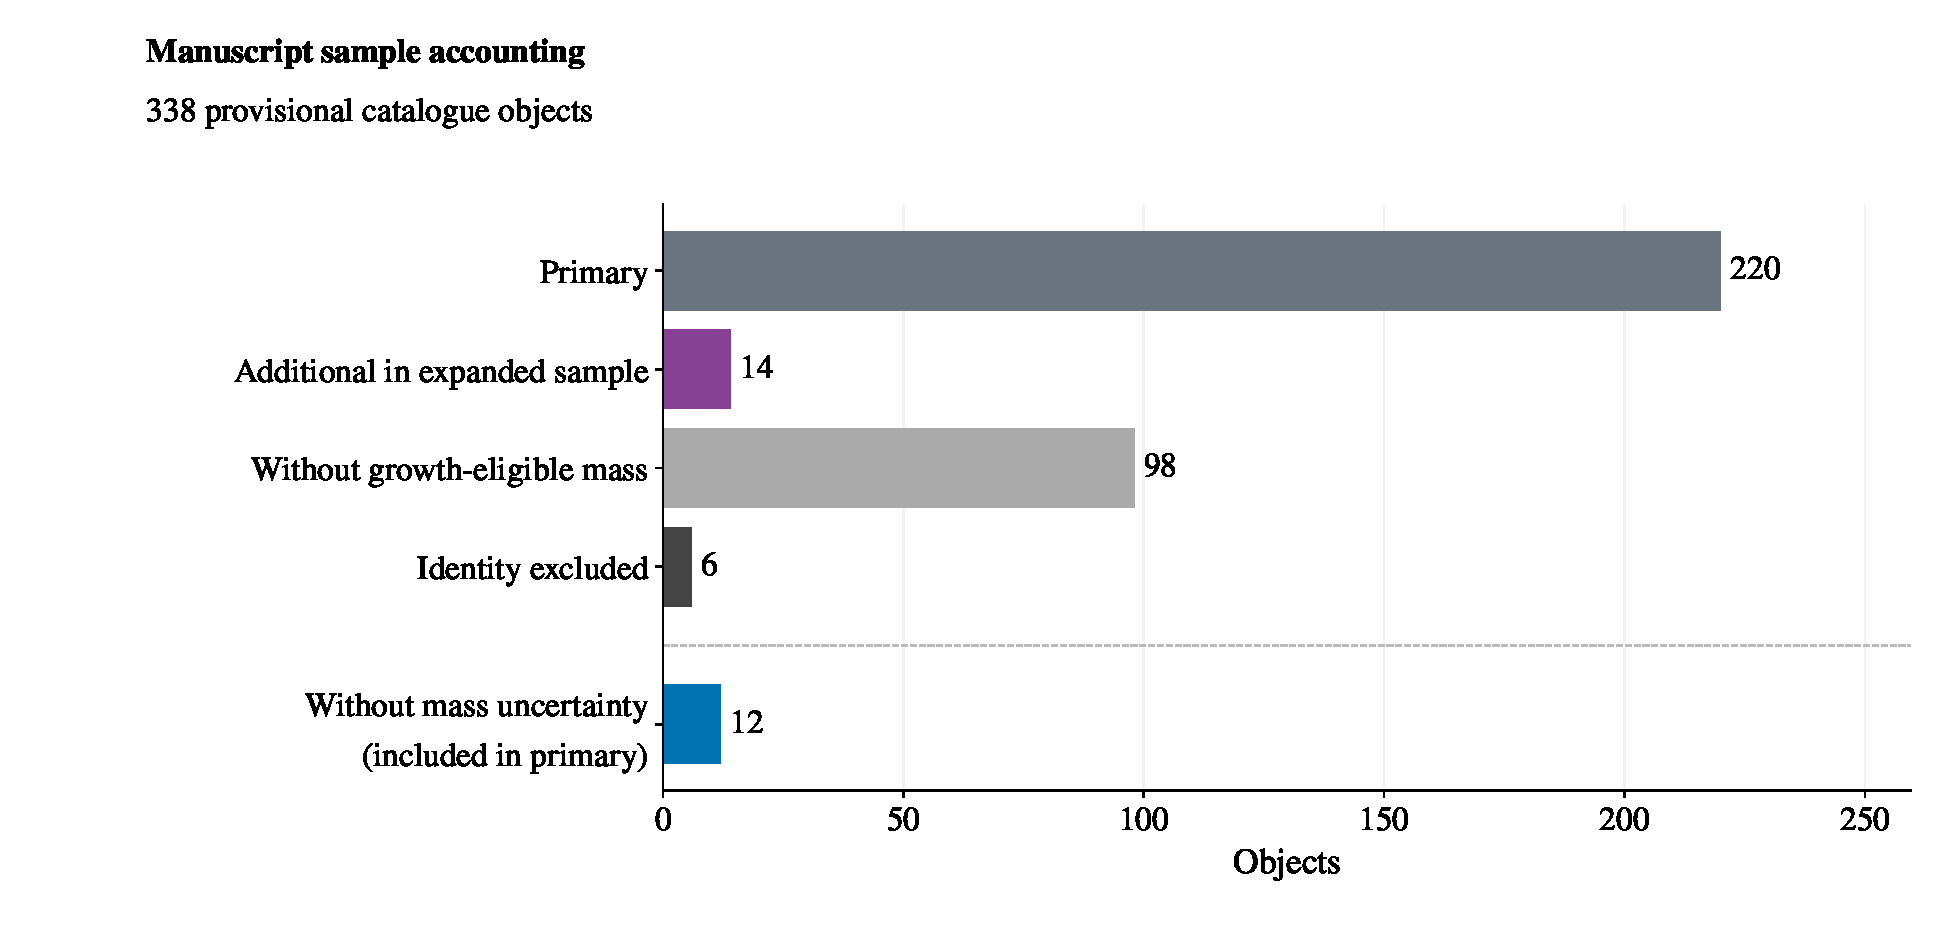
\includegraphics[width=0.92\textwidth]{figures/landscape.pdf}
\captionof{figure}{Sample accounting for 343 provisional catalogue objects. The first four
bars show mutually exclusive categories: 223 primary objects, 15 additional
expanded-sample objects, 99 retained without eligible masses, and 6 identity exclusions.
The final bar shows the 12 primary objects without reported mass uncertainties;
these are included in the primary count. The expanded sample contains
238 objects. Probability calculations use 211 primary and 226 expanded-sample objects.}
\label{fig:landscape}
\end{minipage}

\par\bigskip
\noindent\begin{minipage}{\textwidth}
\centering
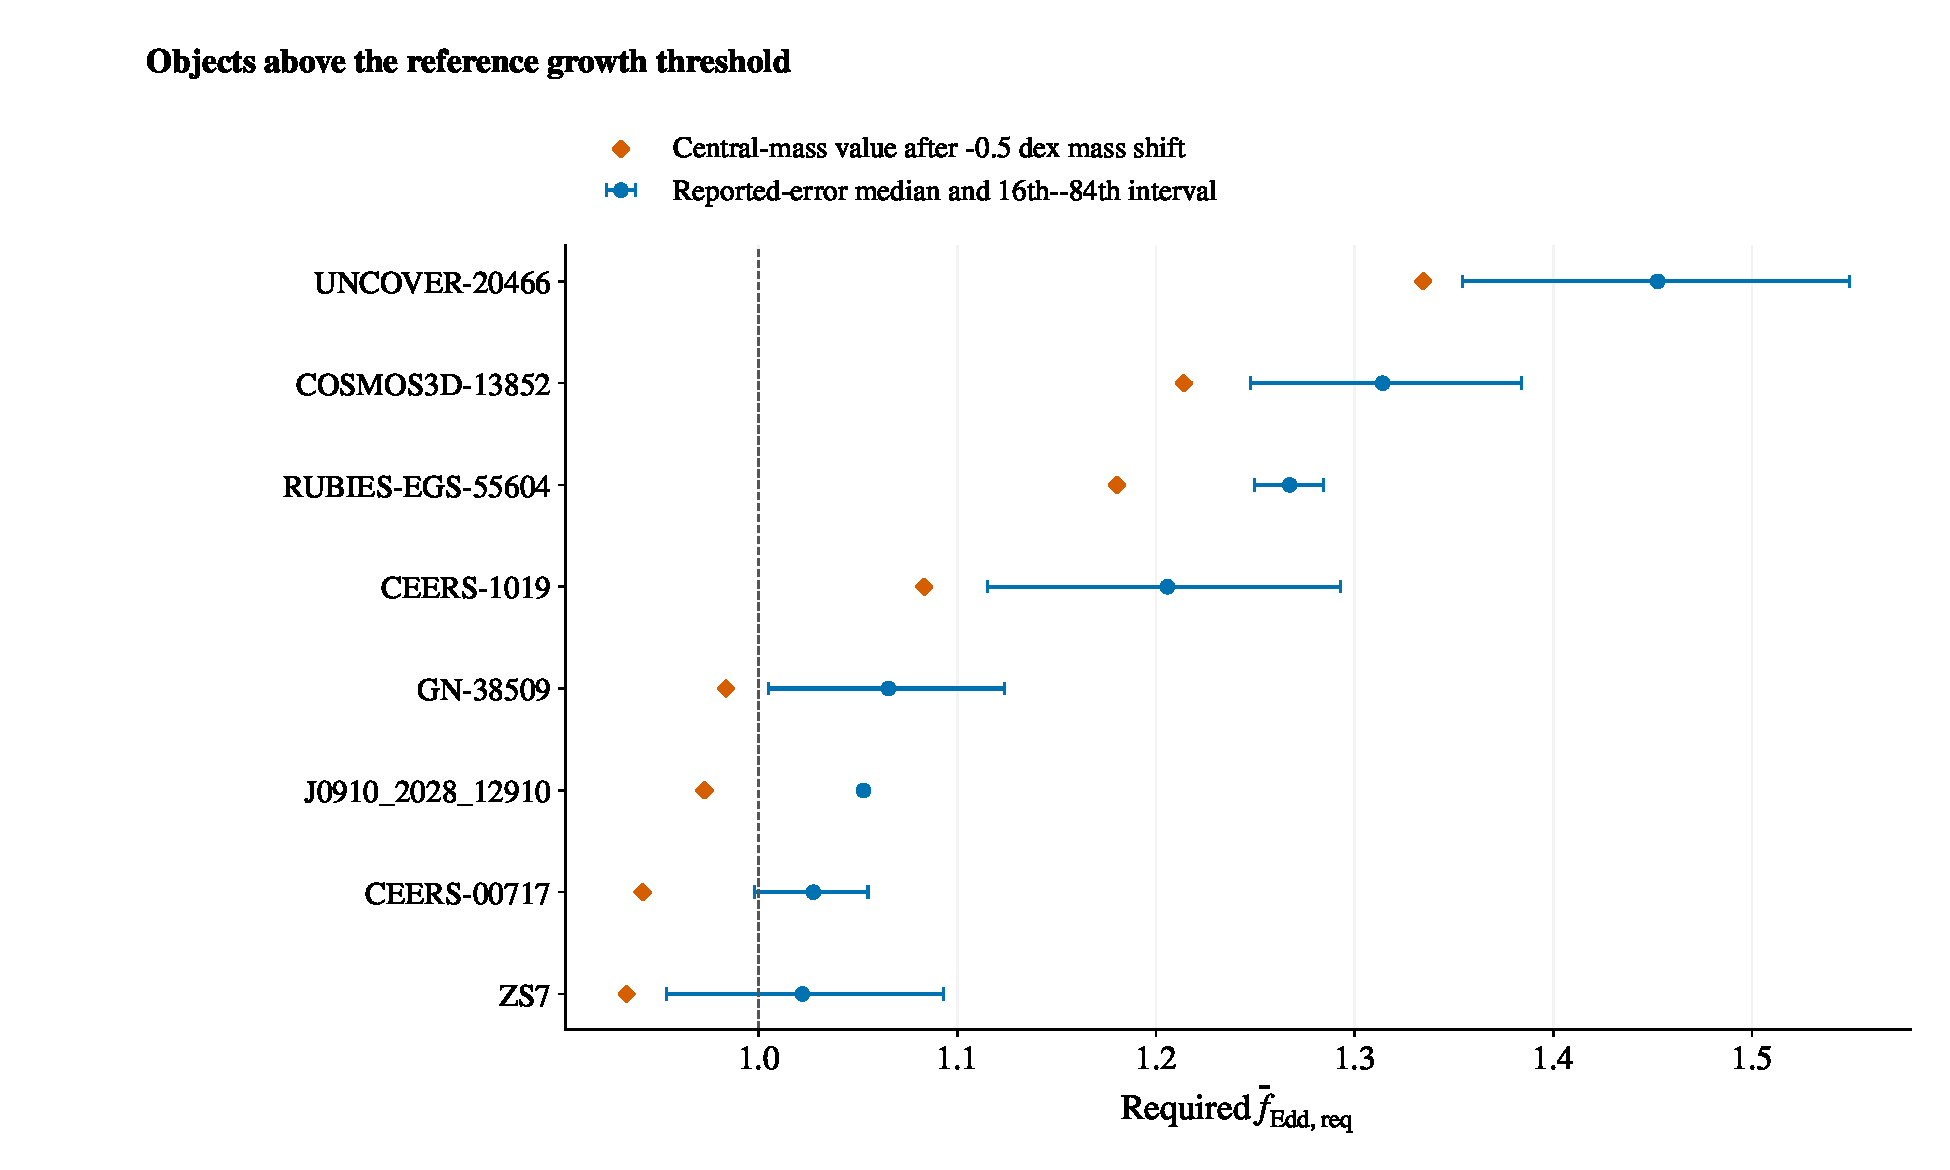
\includegraphics[width=0.92\textwidth]{figures/uncertainty.pdf}
\captionof{figure}{The eleven primary objects with $f_0>1$, where $f_0$ is the
required lifetime-average Eddington ratio at the adopted central mass under
the reference model. Circles and bars show medians and 16th--84th percentile intervals of the
required lifetime-average Eddington ratio over each object's mass-error draws;
diamonds show $f_0$ after a $-0.5$ dex mass shift. The vertical
line is the reference threshold. The selected objects all have reported errors;
these intervals do not include additional estimator systematics.}
\label{fig:uncertainty}
\end{minipage}

\par\bigskip
\noindent\begin{minipage}{\textwidth}
\centering
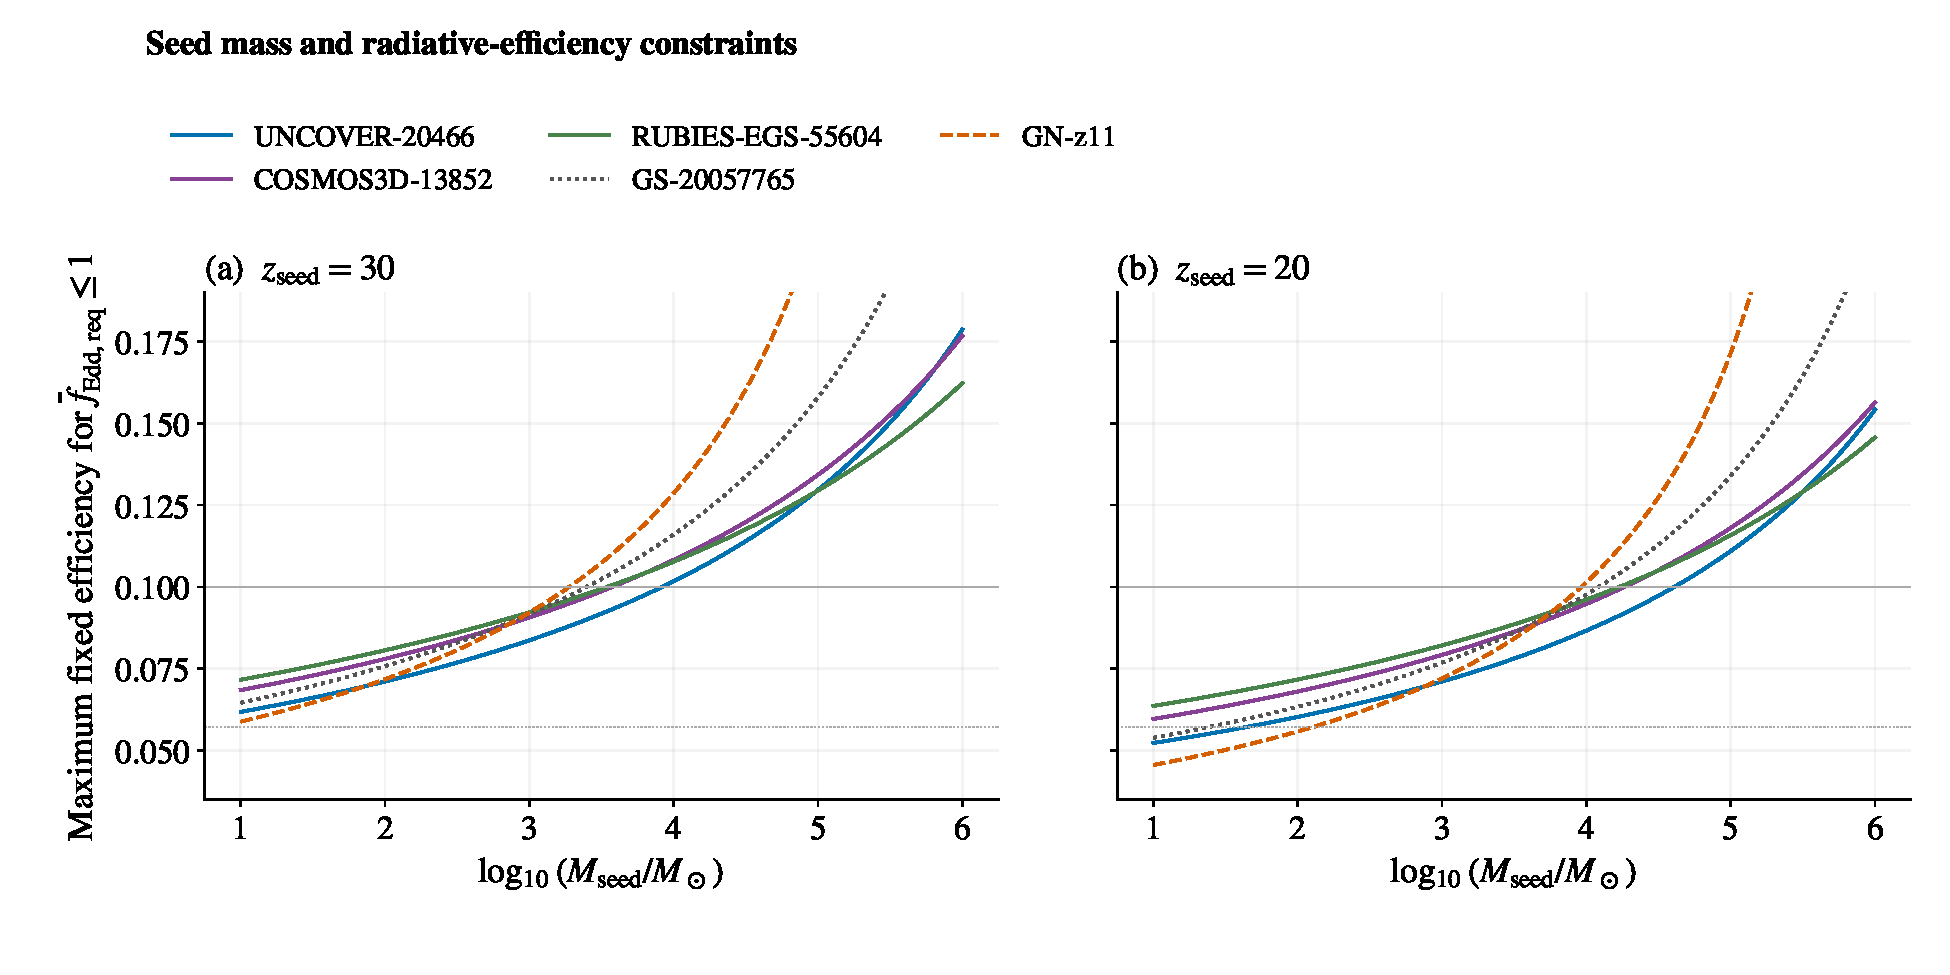
\includegraphics[width=0.92\textwidth]{figures/growth_boundaries.pdf}
\captionof{figure}{Seed-mass--efficiency boundaries for Eddington-limited average growth
at 2 starting redshifts. Each curve uses an adopted central mass and no merger
boost. Below a curve the required average is at most unity. Horizontal guides
mark $\epsilon=0.1$ (solid grey) and $0.05719$ (dotted grey).
The targets are the five primary objects retaining $P\geq0.95$ after a
$-0.5$ dex mass shift under the reported-error model, and GN-z11 from the
expanded sample.
Each point assumes a radiative efficiency that remains constant throughout growth.}
\label{fig:boundaries}
\end{minipage}

\par\bigskip
\noindent\begin{minipage}{\textwidth}
\centering
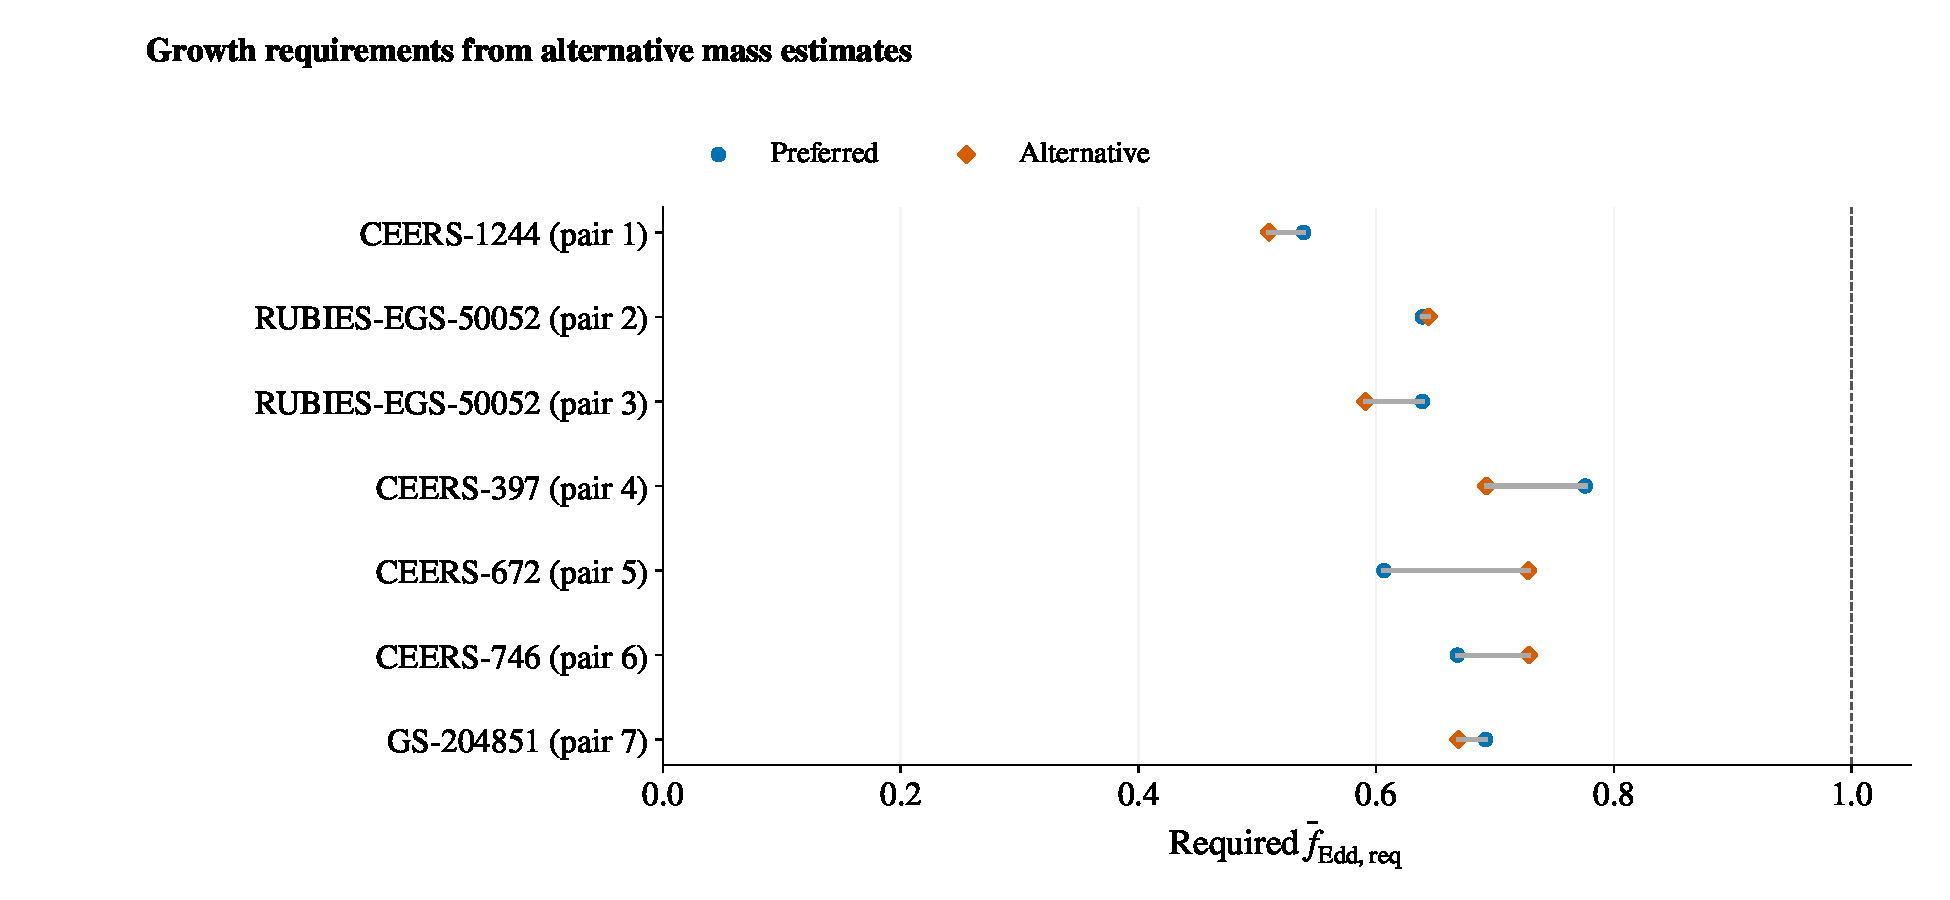
\includegraphics[width=0.99\textwidth]{figures/measurement_sensitivity.pdf}
\captionof{figure}{Preferred (circles) and alternative (diamonds) required ratios at the central masses for
7 measurement pairs across 6 primary objects. Pair numbers follow the
released alternative-measurement table, which supplies stable measurement identifiers;
RUBIES-EGS-50052 (CEERS-2782) has 2 alternatives. All pairs remain below the reference threshold.}
\label{fig:sensitivity}
\end{minipage}

\par\bigskip
\noindent\begin{minipage}{\textwidth}
\centering
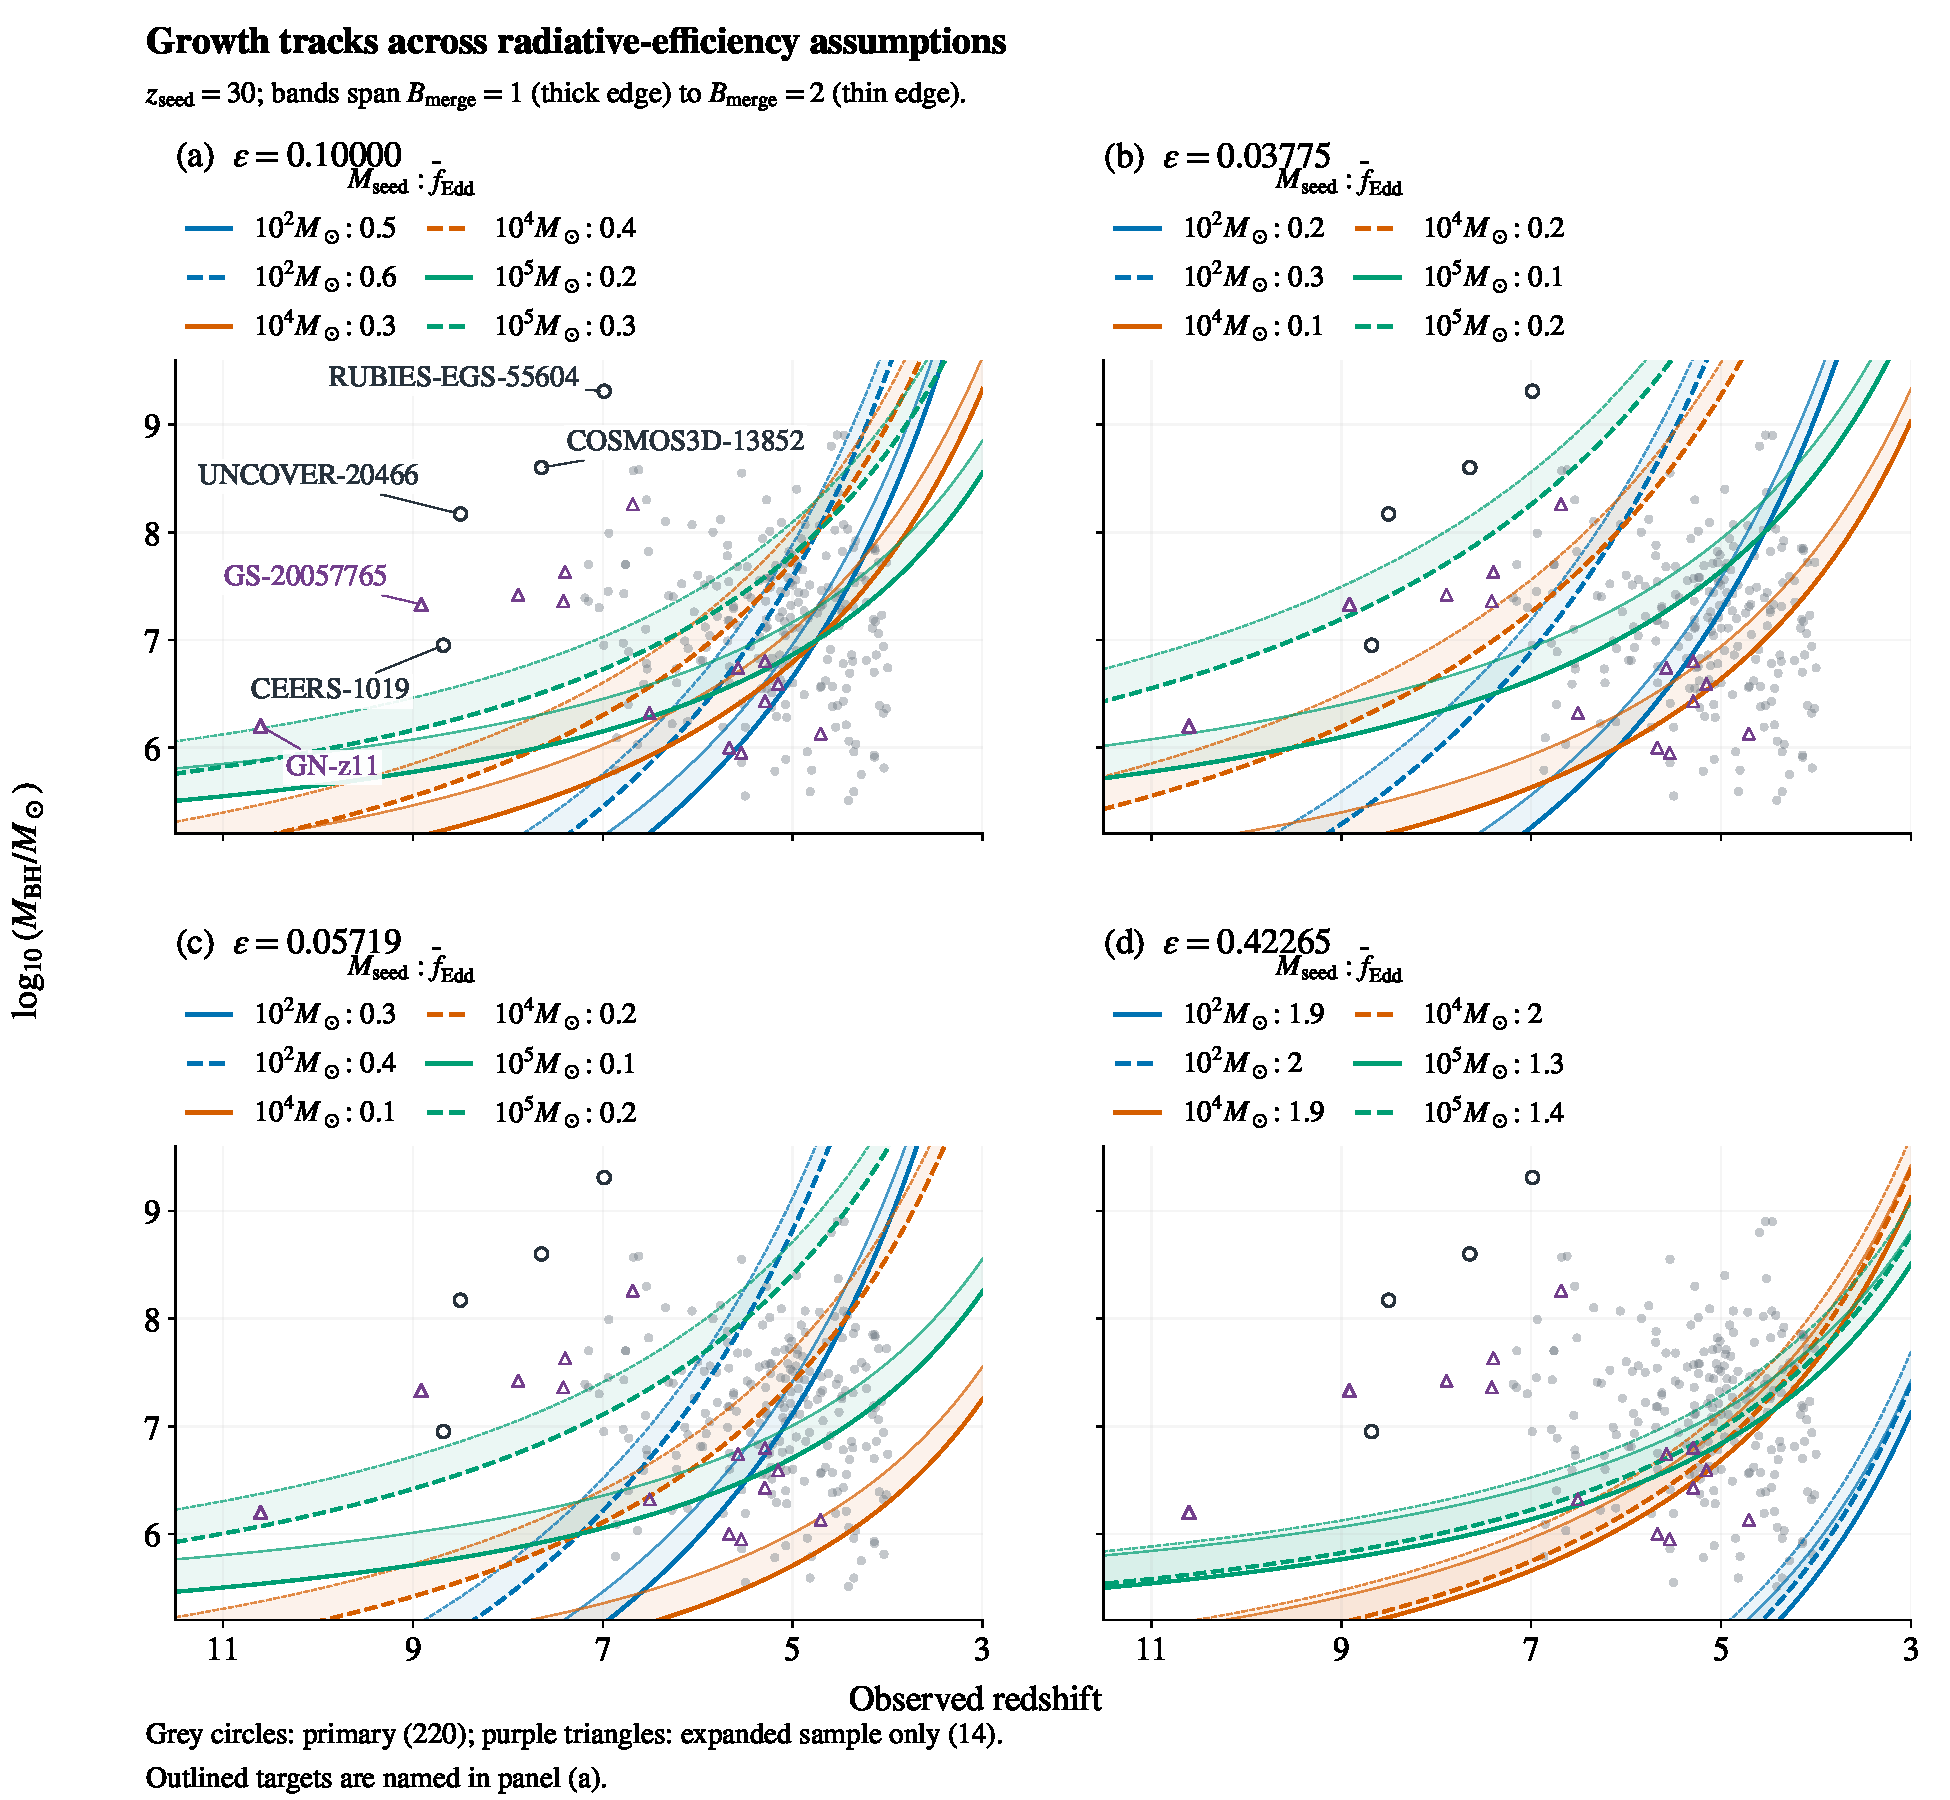
\includegraphics[width=0.99\textwidth]{figures/growth_tracks.pdf}
\captionof{figure}{Growth tracks with 223 primary and 15 additional objects.
Panels show 4 constant radiative efficiencies at $z_{\rm seed}=30$;
colours distinguish seeds of $10^2$, $10^4$, and $10^5M_\odot$, and legends
list the average Eddington ratios, selected separately in each panel to lie
near the sample. Shaded bands span merger boosts
$B_{\rm merge}=1$--2, with thick and thin edges respectively.
The five primary objects retaining $P\geq0.95$ after a $-0.5$ dex mass shift
under the reported-error model, together with GN-z11, are labelled in the
first panel and highlighted in every panel.
Objects with unresolved identities or without eligible masses are omitted.}
\label{fig:allgrowth}
\end{minipage}

\par\bigskip
\noindent\begin{minipage}{\textwidth}
\centering
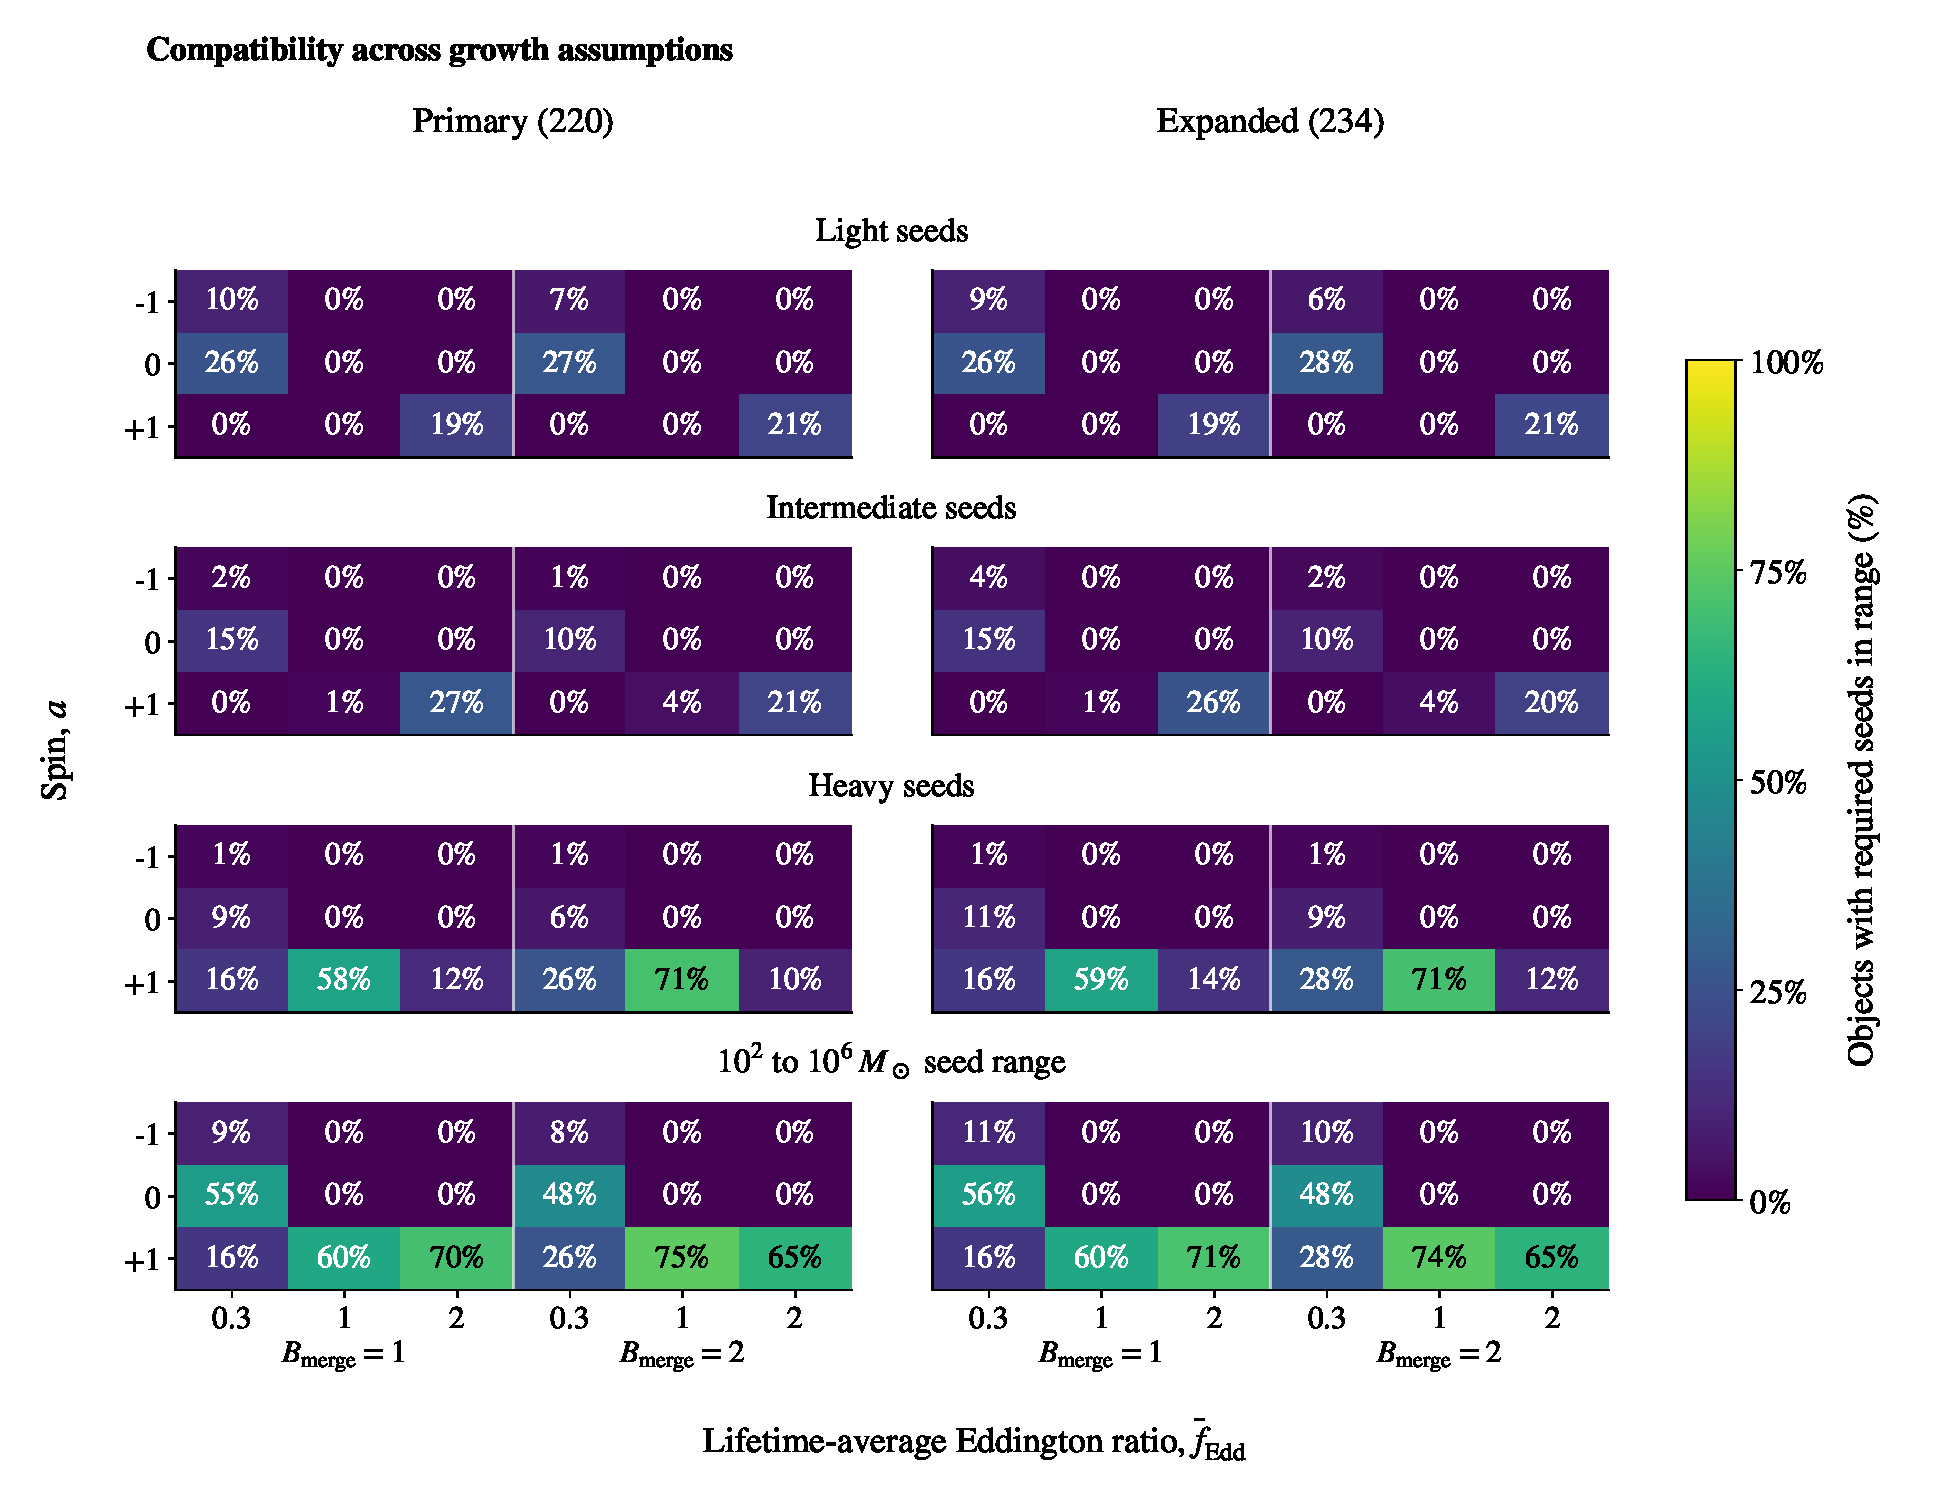
\includegraphics[width=0.99\textwidth]{figures/compatibility.pdf}
\captionof{figure}{Constant-state compatibility fractions in the primary
sample (left) and the expanded sample (right). The expanded sample includes all primary objects. Each column specifies merger multiplier $B_{\rm merge}$ and fixed luminosity
ratio $\fedd$; rows specify ideal spin-dependent efficiency, with the supercritical
prescription in Section~\ref{app:efficiency}. Seed intervals overlap and have no assigned probability weights.}
\label{fig:compatibility}
\end{minipage}

\par\bigskip
\noindent\begin{minipage}{\textwidth}
\centering
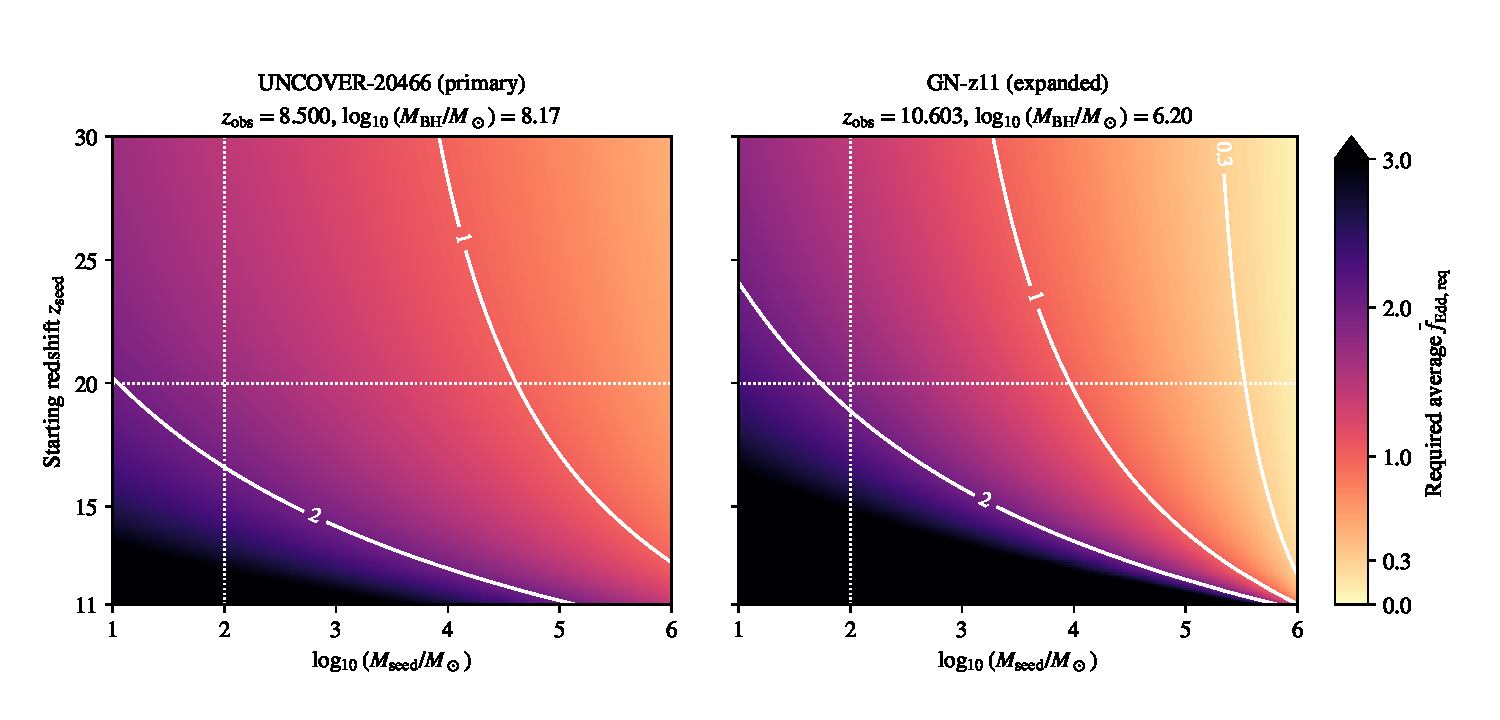
\includegraphics[width=0.99\textwidth]{figures/seed_timing_comparison.pdf}
\captionof{figure}{Required average Eddington ratio for UNCOVER-20466 (primary sample)
and GN-z11 (expanded sample), using their adopted central masses and
redshifts shown above each panel. Both panels use $\epsilon=0.1$, no merger
boost, and the same axes and colour scale. White contours mark required
ratios of 0.3, 1, and 2; dotted guides mark a $100\,M_\odot$ seed and
$z_{\rm seed}=20$. Colours saturate above a required ratio of 3.
Mass uncertainties are not propagated in these maps.}
\label{fig:seed-timing}
\end{minipage}

\par\bigskip
\noindent\begin{minipage}{\textwidth}
\centering
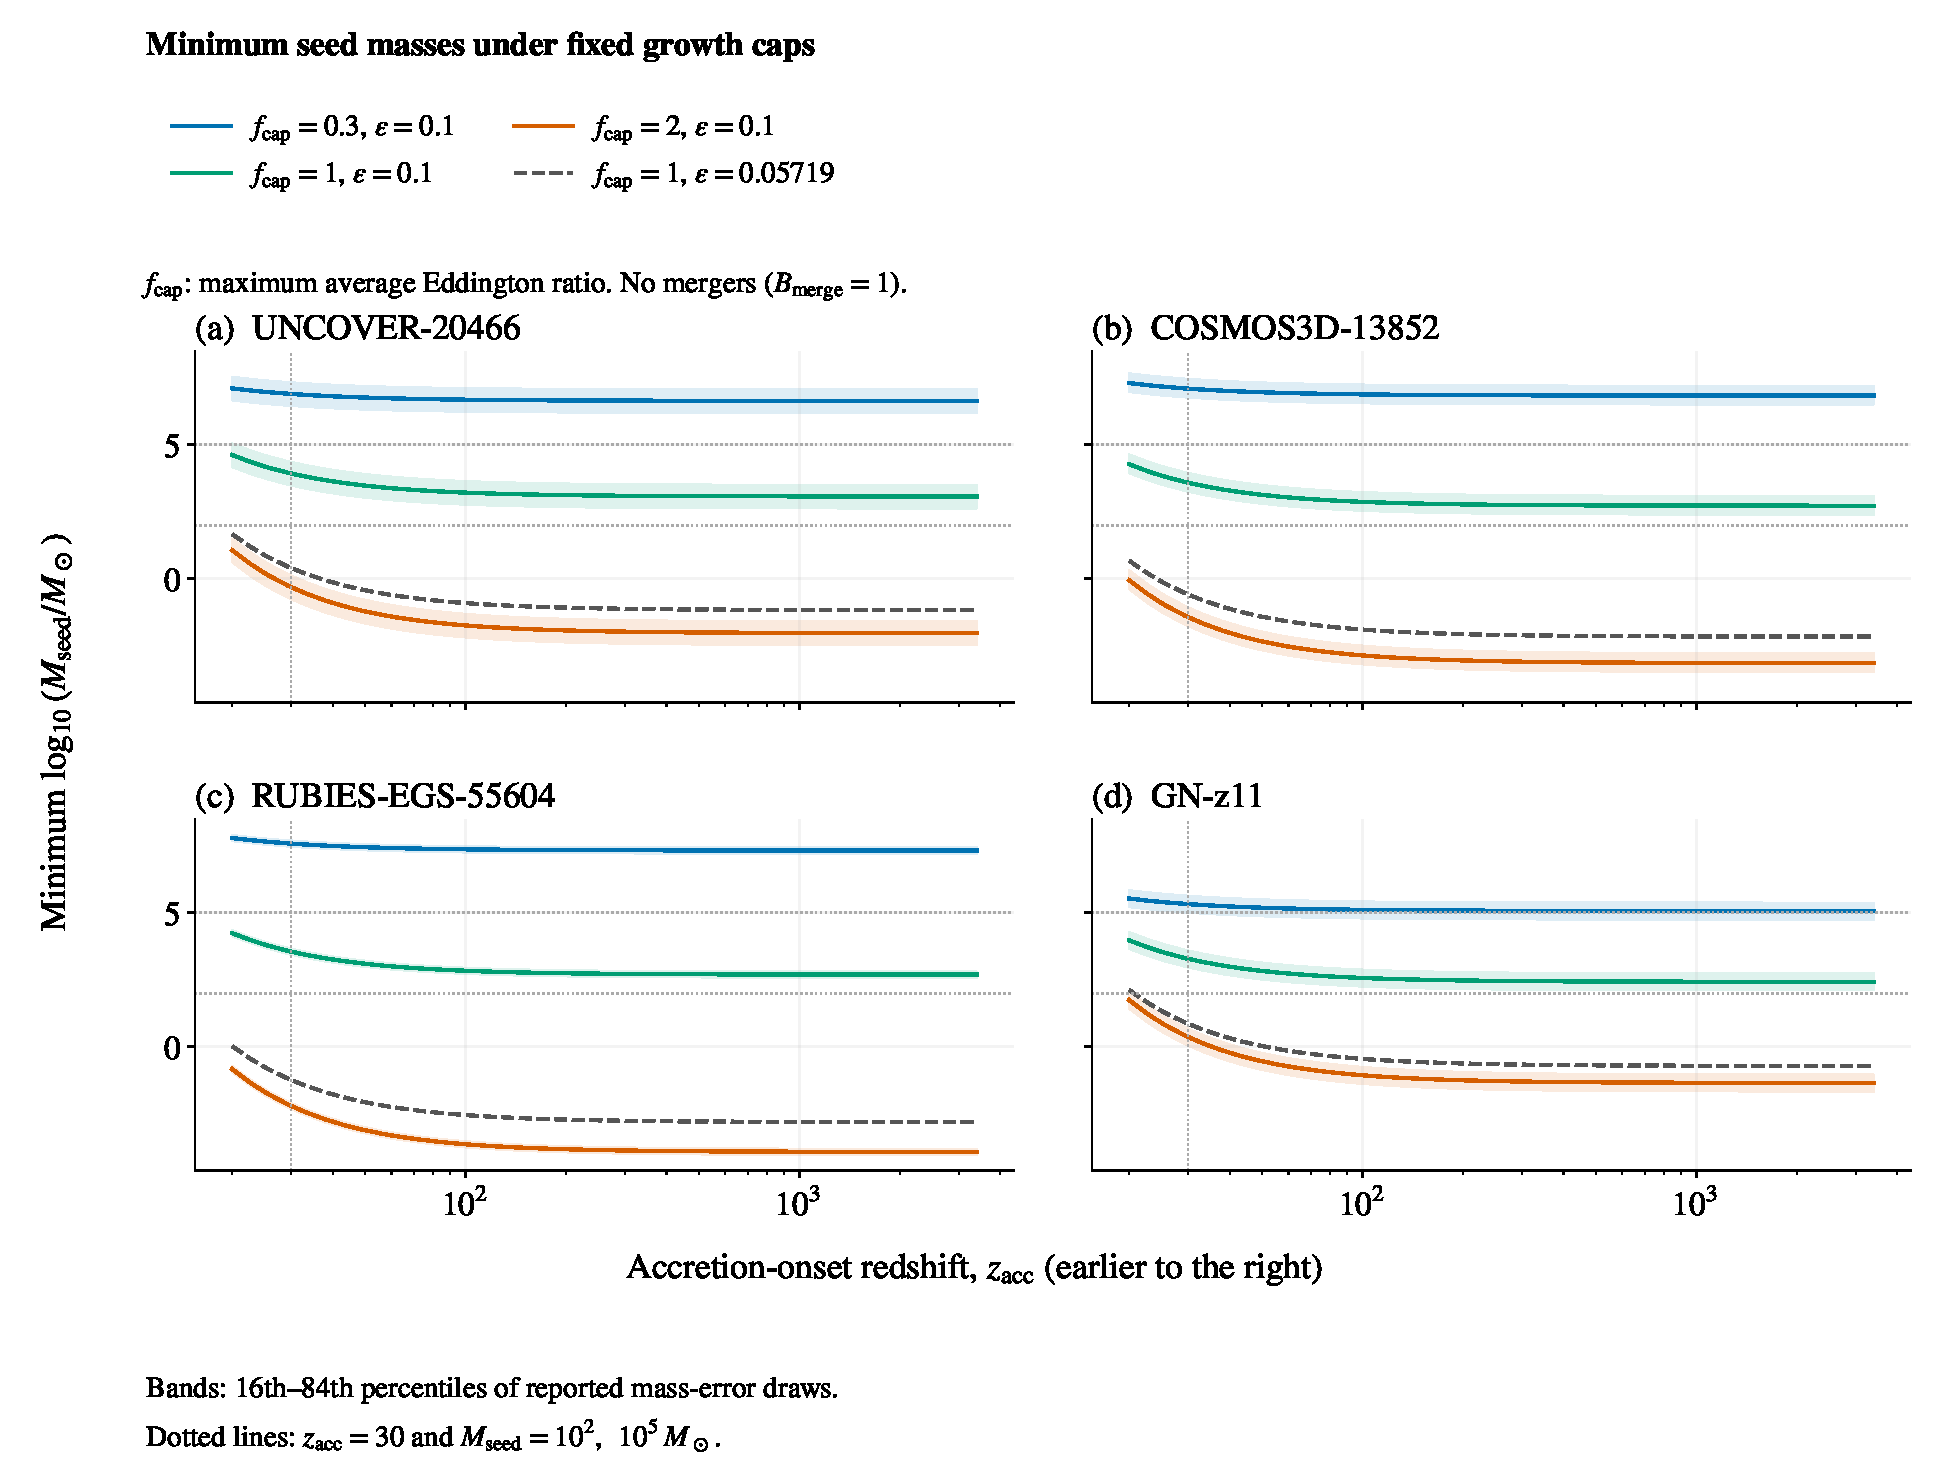
\includegraphics[width=0.99\textwidth]{figures/v4_minimum_seed_mass.pdf}
\captionof{figure}{Minimum onset seed mass versus accretion-onset redshift for the four
targets. Solid curves vary the average Eddington-ratio cap at fixed
$\epsilon=0.1$; shaded bands propagate the 16th--84th percentiles of reported
mass errors. Dashed curves show the lower-efficiency sensitivity. Earlier
onset reduces the required mass, with diminishing gains in available time.}
\label{fig:pbh-minimum}
\end{minipage}

\clearpage
\section*{Tables}
\noindent\begin{minipage}{\textwidth}
\centering\captionof{table}{\textbf{Catalogue contents and analysis samples.} Measurements are
literature records of individual objects; an object may have records from
several studies. Object counts are provisional where identifications across
studies remain uncertain.}
\begin{tabular}{@{}lr@{}}
\toprule
Category & Count \\
\midrule
Measurements / provisional objects / host systems & 355 / 343 / 342 \\
Growth-eligible measurements / objects & 248 / 241 \\
Preliminary Balmer selection: measurements / objects & 237 / 230 \\
Primary sample / expanded sample & 223 / 238 \\
Objects with mass uncertainties (primary / expanded) & 211 / 226 \\
Objects excluded for uncertain identity & 6 \\
Objects without growth-eligible measurements & 102 \\
\bottomrule
\end{tabular}
\par\smallskip
\parbox{\textwidth}{\footnotesize
The preliminary Balmer selection requires a non-conditional Balmer virial mass and
secure or probable evidence for an accreting black hole in the catalogue.
These counts precede the final checks of individual line detections and object identities.
Of these 230 objects, 4 tentative JADES detections enter
only the expanded sample and 3 are excluded for uncertain identity,
leaving 223 primary objects. The 102 objects without eligible masses include
3 of the 6 identity exclusions. Figure~\ref{fig:landscape} counts those 3
under identity exclusions, leaving 99 in its bar for objects without eligible masses.}
\label{tab:scale}
\end{minipage}

\par\bigskip
\begingroup\footnotesize
\setlength{\tabcolsep}{4pt}
\begin{longtable}{@{}>{\raggedright\arraybackslash}p{0.27\textwidth}rp{0.10\textwidth}>{\raggedright\arraybackslash}p{0.43\textwidth}@{}}
\caption{Source-family inventory. Counts are catalogue measurements / growth-eligible
measurements / primary-sample objects (M/E/P).
The columns sum to 355/248/223; E includes alternatives, whereas P counts each
selected object once. ``Balmer'' denotes single-epoch virial masses.
``Context'' denotes mass estimates retained for discussion but excluded from
growth calculations because of their method or interpretation.
``Upper limit'' denotes an upper bound rather than a measured central mass;
these bounds are also excluded from growth calculations.
}
\label{tab:sources}\\
\toprule Source & M/E/P & Mass & Selection channel; principal caveat \\\midrule
\endfirsthead
\multicolumn{4}{l}{Table~\ref{tab:sources} continued}\\
\toprule Source & M/E/P & Mass & Selection channel; principal caveat \\\midrule
\endhead
\bottomrule\endfoot
\tableinput{tables/source_rows.tex}
\end{longtable}
\endgroup

\par\bigskip
\noindent\begin{minipage}{\textwidth}
\centering
\captionof{table}{Core growth-testing coverage for the admissible expanded sample.
Counts exclude objects without eligible masses, unresolved-identity exclusions,
and status-only records. Per-object counts refer to the same adopted mass
under different assumptions; grid points are numerical evaluations, not
independent physical models.}
\begin{tabular}{@{}>{\raggedright\arraybackslash}p{0.48\textwidth}rr@{}}
\toprule
Product & Per object & Sample total \\
\midrule
Required accretion rates & 3 & 714 \\
Required seed masses & 2 & 476 \\
Duty-cycle requirements & 3 & 714 \\
Growth compatibility checks & 72 & 17,136 \\
Four core tabulated products & 80 & 19,040 \\
Numerical parameter maps & 2 & 476 \\
Seed--accretion grid evaluations & 54,000 & 12,852,000 \\
Seed--onset grid evaluations & 22,500 & 5,355,000 \\
Combined grid evaluations & 76,500 & 18,207,000 \\
Monte Carlo mass draws$^{\rm a}$ & 10,000 & 2,260,000 \\
\bottomrule
\end{tabular}
\par\smallskip
\parbox{\textwidth}{\footnotesize
The expanded sample has 238 objects, including 223 primary objects.
The additional summary, availability, comparison, and minimum-seed tables
in Section~\ref{sec:products} are counted separately.
$^{\rm a}$ Only the 226 expanded-sample objects with reported mass errors are
sampled; the other 12 enter central-mass calculations only. The primary
sample alone contributes 17,059,500 map-grid evaluations and 2,110,000 mass
draws for its 211 objects with errors. The archival release additionally
retains numerical entries for 3 identity-excluded objects and status records
for 102 objects without eligible masses; none contributes to the counts here.
The four-target earlier-onset extension has 2,256 minimum-seed results,
12,408 seed--onset map entries, and 288 control entries, reported separately
(Appendix~\ref{sec:pbh-v4}).}
\label{tab:products}
\end{minipage}


\par\bigskip
\noindent\begin{minipage}{\textwidth}
\centering
\captionof{table}{The eleven primary objects above the reference threshold, ordered by $f_0$.
Redshifts are the adopted spectroscopic values. Masses and errors are in
$\log_{10}(\mbh/M_\odot)$; all estimators are single-epoch
virial. $f_0$ is the required lifetime-average Eddington ratio evaluated
at the adopted central mass under the reference model; $f_{16}$ is the
16th percentile of this required ratio over the object's mass-error draws,
and $P_0=P(\overline{f}_{\mathrm{Edd,req}}>1)$.
$f_-$ and $P_-$ apply the fixed $-0.5$ dex offset. $\Delta m$ (dex) is the
reduction in log mass that brings the central required average Eddington
ratio to 1, with the growth assumptions unchanged. All probabilities use
the quoted mass errors and fixed growth assumptions. Additional mass-estimator limitations are in Table~\ref{tab:actions}.}
\begingroup\small\setlength{\tabcolsep}{3pt}
\begin{tabular}{@{}>{\raggedright\arraybackslash}p{0.245\textwidth}rlrrrrrrr@{}}
\toprule
Object/source & $z$ & Line & Log mass & $f_0$ & $f_{16}$ & $P_0$ & $f_-$ & $P_-$ & $\Delta m$ \\
\midrule
\tableinput{tables/target_rows.tex}
\bottomrule
\end{tabular}
\par\smallskip
\parbox{\textwidth}{\footnotesize
$^{\rm a}$ A separate 0.5-dex calibration scale is reported for
\mbox{RUBIES-EGS-55604} and J0910\_2028\_12910; these scales are omitted from the
quoted errors and probabilities shown here. $^{\rm b}$ GN-38509's quoted
mass errors already include 0.3-dex calibration scatter. $^{\rm c}$ ZS7's quoted 0.4-dex error
already includes calibration scatter. $^{\rm d}$ J1007\_AGN has a separate
0.43-dex calibration scale, omitted here and tested in Table~\ref{tab:calibration}.
Unmarked rows have no separate scalar
numerical calibration scale recorded; their quoted errors may omit other
mass-estimator uncertainties.}
\endgroup
\label{tab:top}
\end{minipage}

\par\bigskip
\noindent\begin{minipage}{\textwidth}
\centering
\captionof{table}{Sensitivity to fixed mass offsets under the reference model.
The slash-separated counts are for objects above unity at the central mass, at the 16th percentile,
and with conditional $P(\overline{f}_{\mathrm{Edd,req}}>1)\geq0.95$.
The probability-based counts use 211 primary and 226 expanded-sample objects with
reported errors; central-mass counts use all 223 and 238 objects.}
\begin{tabular}{@{}lrr@{}}
\toprule
Mass offset (dex) & Primary & Expanded \\
\midrule
$-0.5$ & 7 / 5 / 5 & 10 / 7 / 6 \\
$-0.3$ & 9 / 8 / 6 & 13 / 10 / 7 \\
$0$ & 11 / 9 / 8 & 17 / 13 / 11 \\
$+0.3$ & 14 / 14 / 13 & 21 / 18 / 17 \\
$+0.5$ & 18 / 15 / 14 & 25 / 21 / 18 \\
\bottomrule
\end{tabular}
\label{tab:massoffset}
\end{minipage}

\par\bigskip
\noindent\begin{minipage}{\textwidth}
\centering
\captionof{table}{Conditional probabilities of exceeding the reference required
average Eddington ratio of 1. Reported-error probabilities use the adopted
error models without Monte Carlo sampling. The calibration columns add
independent Gaussian scatter: 0.5 dex for RUBIES-EGS-55604 and
J0910\_2028\_12910, and 0.43 dex for J1007\_AGN. The symmetric cases use
exact normal tails; J1007's asymmetric errors use numerical convolution.
The baseline Monte Carlo results and sample membership are unchanged.}
\begin{tabular}{@{}lrrrr@{}}
\toprule
& \multicolumn{2}{c}{No mass shift} & \multicolumn{2}{c}{$-0.5$ dex shift} \\
Object & Reported & + calibration & Reported & + calibration \\
\midrule
\tableinput{tables/calibration_rows.tex}
\bottomrule
\end{tabular}
\label{tab:calibration}
\end{minipage}

\par\bigskip
\noindent\begin{minipage}{\textwidth}
\centering
\captionof{table}{Objects requiring $\overline{f}_{\mathrm{Edd,req}}>1$ at their central
masses under fixed growth assumptions. Each row changes only the named parameter from the reference
($M_{\rm seed}=10^2M_\odot$, $z_{\rm seed}=30$, $\epsilon=0.1$,
$B_{\rm merge}=1$). Counts use central mass estimates and provisional object identities.}
\begin{tabular}{@{}lrr@{}}
\toprule
Scenario & Primary (223) & Expanded (238) \\
\midrule
Reference & 11 & 17 \\
$M_{\rm seed}=10^3M_\odot$ & 5 & 7 \\
$M_{\rm seed}=10^5M_\odot$ & 0 & 0 \\
$z_{\rm seed}=20$ & 21 & 28 \\
$\epsilon=0.05719$ & 0 & 0 \\
\bottomrule
\end{tabular}
\label{tab:scenarios}
\end{minipage}

\par\bigskip
\noindent\begin{minipage}{\textwidth}
\centering\small
\captionof{table}{Mass-estimator limitations for the 11 primary objects requiring
$\overline{f}_{\mathrm{Edd,req}}>1$ under the reference assumptions.
Caveats summarize the source records cited in Table~\ref{tab:top}.}
\begin{tabular}{@{}>{\raggedright\arraybackslash}p{0.28\textwidth}>{\raggedright\arraybackslash}p{0.68\textwidth}@{}}
\toprule
Object & Mass-estimator caveat \\
\midrule
CAPERS-LRD-z9 & H$\beta$; dense gas and broad-line-region geometry, correlated dust alternatives; the 0.15 dex error includes calibration coefficients but not the full high-redshift systematic. \\[3pt]
CANUCS-LRD-z8.6 & H$\beta$; mass already lens-corrected; alternate lens model and calibration-scatter decomposition remain caveats. \\[3pt]
J1007\_AGN & Observed total-H$\beta$ luminosity estimator; correlated dust correction raises the mass; separate 0.43 dex calibration scale tested in Table~\ref{tab:calibration}. \\[3pt]
UNCOVER-20466 & H$\beta$; mass depends on lens model and broad-line-region interpretation. \\[3pt]
COSMOS3D-13852 & H$\beta$; possible scattering bias; 1--2 dex shifts tested here. \\[3pt]
\mbox{RUBIES-EGS-55604} & H$\beta$; dust-corrected mass; separate 0.5 dex calibration scale. \\[3pt]
CEERS-1019 & Weak broad H$\beta$ component. \\[3pt]
GN-38509 & H$\alpha$; quoted mass errors include 0.3 dex calibration scatter. \\[3pt]
J0910\_2028\_12910 & H$\alpha$; 0.01 dex formal error excludes a 0.5 dex calibration scale. \\[3pt]
CEERS-00717 & H$\alpha$; local calibration; no quantitative systematic uncertainty reported. \\[3pt]
ZS7 & H$\beta$; quoted 0.4 dex already includes calibration scatter. \\[3pt]
\bottomrule
\end{tabular}
\label{tab:actions}
\end{minipage}

\par\bigskip
\noindent\begin{minipage}{\textwidth}
\centering\small
\captionof{table}{Effect of replacing the adopted Baccus preprint values with published measurements,
with unresolved identities excluded throughout. Counts denote required ratios
above unity at the central masses, 16th percentiles above unity, and conditional $P\geq0.95$,
respectively. The adopted catalogue values define the baseline.}
\begin{tabular}{@{}llrr@{}}
\toprule
Sample & Measurement treatment & Objects & Counts \\
\midrule
Primary & Adopted catalogue values & 223 & 11/9/8 \\
Primary & Published; retain unmatched & 223 & 11/9/8 \\
Primary & Published; omit unmatched & 219 & 11/9/8 \\
Expanded & Adopted catalogue values & 238 & 17/13/11 \\
Expanded & Published; retain unmatched & 238 & 17/13/11 \\
Expanded & Published; omit unmatched & 234 & 17/13/11 \\
\bottomrule
\end{tabular}
\label{tab:baccusjoint}
\end{minipage}

\par\bigskip
\noindent\begin{minipage}{\textwidth}
\centering
\captionof{table}{Minimum onset seed masses ($M_\odot$) for the four targets at
their adopted central masses, $\epsilon=0.1$, $f_{\rm cap}=1$, and no mergers.
All columns use radiation-inclusive cosmic ages. Values are rounded;
Figure~\ref{fig:pbh-minimum} shows the reported-error sensitivity.}
\begin{tabular}{@{}lrrr@{}}
\toprule
Object & $z_{\rm acc}=30$ & $z_{\rm acc}=100$ & $z_{\rm acc}=3400$ \\
\midrule
\tableinput{tables/v4_seed_requirements.tex}
\bottomrule
\end{tabular}
\label{tab:pbh-seeds}
\end{minipage}

\end{document}
